%% This is file `elsarticle-template-1-num.tex',
%%
%% Copyright 2009 Elsevier Ltd
%%
%% This file is part of the 'Elsarticle Bundle'.
%% ---------------------------------------------
%%
%% It may be distributed under the conditions of the LaTeX Project Public
%% License, either version 1.2 of this license or (at your option) any
%% later version.  The latest version of this license is in
%%    http://www.latex-project.org/lppl.txt
%% and version 1.2 or later is part of all distributions of LaTeX
%% version 1999/12/01 or later.
%%
%% The list of all files belonging to the 'Elsarticle Bundle' is
%% given in the file `manifest.txt'.
%%
%% Template article for Elsevier's document class `elsarticle'
%% with numbered style bibliographic references
%%
%% $Id: elsarticle-template-1-num.tex 149 2009-10-08 05:01:15Z rishi $
%% $URL: http://lenova.river-valley.com/svn/elsbst/trunk/elsarticle-template-1-num.tex $
%%

%\documentclass[preprint,authoryear,review,12pt]{elsarticle}
\documentclass[final,5p,times,twocolumn]{elsarticle}

%% Use the option review to obtain double line spacing
%% \documentclass[preprint,review,12pt]{elsarticle}

%% Use the options 1p,two column; 3p; 3p,twocolumn; 5p; or 5p,twocolumn
%% for a journal layout:
%% \documentclass[final,1p,times]{elsarticle}
%% \documentclass[final,1p,times,twocolumn]{elsarticle}
%% \documentclass[final,3p,times]{elsarticle}
%% \documentclass[final,3p,times,twocolumn]{elsarticle}
%% \documentclass[final,5p,times]{elsarticle}
%% \documentclass[final,5p,times,twocolumn]{elsarticle}


\usepackage{color}
\usepackage{multirow,booktabs,ctable,array}
\usepackage{lscape}
\usepackage{amsmath}
\usepackage{lineno}
\usepackage{ulem}
\usepackage{setspace}
\usepackage{listings}
\usepackage{float}


\floatstyle{plain}
\newfloat{command}{thp}{lop}
\floatname{command}{Command}

%\usepackage[nomarkers,notablist]{endfloat}

%% if you use PostScript figures in your article
%% use the graphics package for simple commands
%% \usepackage{graphics}
%% or use the graphicx package for more complicated commands
%% \usepackage{graphicx}
%% or use the epsfig package if you prefer to use the old commands
%% \usepackage{epsfig}

%% The amssymb package provides various useful mathematical symbols
\usepackage{amssymb}
%% The amsthm package provides extended theorem environments
% \usepackage{amsthm}
 
 \usepackage{makecell}

%% The lineno packages adds line numbers. Start line numbering with
%% \begin{linenumbers}, end it with \end{linenumbers}. Or switch it on
%% for the whole article with \linenumbers after \end{frontmatter}.
%% \usepackage{lineno}

%% natbib.sty is loaded by default. However, natbib options can be
%% provided with \biboptions{...} command. Following options are
%% valid:

%%   round  -  round parentheses are used (default)
%%   square -  square brackets are used   [option]
%%   curly  -  curly braces are used      {option}
%%   angle  -  angle brackets are used    <option>
%%   semicolon  -  multiple citations separated by semi-colon
%%   colon  - same as semicolon, an earlier confusion
%%   comma  -  separated by comma
%%   numbers-  selects numerical citations
%%   super  -  numerical citations as superscripts
%%   sort   -  sorts multiple citations according to order in ref. list
%%   sort&compress   -  like sort, but also compresses numerical citations
%%   compress - compresses without sorting
%%
%% \biboptions{comma,round}

% \biboptions{}

\providecommand{\OO}[1]{\operatorname{O}\bigl(#1\bigr)}

\graphicspath{{./Figures/}
                          }

\long\def\symbolfootnote[#1]#2{\begingroup%
\def\thefootnote{\fnsymbol{footnote}}\footnote[#1]{#2}\endgroup}

    \usepackage{color}

    \definecolor{listcomment}{rgb}{0.0,0.5,0.0}
    \definecolor{listkeyword}{rgb}{0.0,0.0,0.5}
    \definecolor{listnumbers}{gray}{0.65}
    \definecolor{listlightgray}{gray}{0.955}
    \definecolor{listwhite}{gray}{1.0}

\newcommand{\lstsetcpp}
{
\lstset{frame = tb,
        framerule = 0.25pt,
        float,
        fontadjust,
        backgroundcolor={\color{listlightgray}},
        basicstyle = {\ttfamily\scriptsize},
        keywordstyle = {\ttfamily\color{listkeyword}\textbf},
        identifierstyle = {\ttfamily},
        commentstyle = {\ttfamily\color{listcomment}\textit},
        stringstyle = {\ttfamily},
        showstringspaces = false,
        showtabs = false,
        numbers = none,
        numbersep = 6pt,
        numberstyle={\ttfamily\color{listnumbers}},
        tabsize = 2,
        language=[ANSI]C++,
        floatplacement=!h,
        caption={},
        captionpos=b,
        }
}


\journal{Neuroimage}

\begin{document}


\begin{frontmatter}

\title{Normalization Circularity in Population-Based FA Analysis}



\author[label1]{Nicholas J.~Tustison\fnref{label0}}
%  \ead{ntustison@virginia.edu}
  \fntext[label0]{\scriptsize Corresponding author:  PO Box 801339, Charlottesville, VA 22908; T:  434-924-7730; email address:  ntustison@virginia.edu }
\author[label2]{Brian B.~Avants}
\author[label2]{Philip A.~Cook}
\author[label3]{Junghoon Kim}
\author[label3]{John Whyte}
\author[label2]{James C.~Gee}
\author[label1]{James R.~Stone}

\address[label1]{Department of Radiology and Medical Imaging, University of Virginia, Charlottesville, VA}
\address[label2]{Penn Image Computing and Science Laboratory, University of Pennsylvania,
                Philadelphia, PA}
\address[label3]{Moss Rehabilitation Research Institute, Albert Einstein Healthcare Network, Philadelphia, PA}



%\maketitle

%\linenumbers


\begin{abstract}
Template-based normalization plays a critical role in many population
studies based on diffusion tensor imaging (DTI).  Several current
approaches compute the fractional anisotropy (FA) from the DTI and then
directly register the FA image to a FA template before performing
statistical comparison between different groups within a population.  In
this paper, we demonstrate that this analysis strategy induces selection
bias that varies in strength with the similarity metric used in
registration.  Specifically, we show that the popular sum of squared
difference intensity metric maximizes effect size, rather than
anatomical alignment, and consistently overestimates statistical
significance.  Consequently, we advocate a more traditional approach
that normalizes a population of FA images through the associated T1
anatomical images.  We show that the Symmetric Group Normalization
strategy for unbiased template construction from anatomical (e.g.
T1-weighted) images provides a valid and unbiased coordinate system for
statistical inference of FA differences and yet retains detection power
in comparison to FA-based normalization methods.  We establish this
outcome by using open data comprised of normal controls from the International
Neuroimaging Data-sharing Initiative as well as a cohort of 16 traumatic
brain injury survivors compared with 17 control subjects.  Alignment
comparisons with the normalization component of the popular tract-based
spatial statistics (TBSS) show that our anatomically-based template
approach produces good alignments despite the absence of any direct
FA-to-FA registration.  Of practical consideration we note that the
software tools discussed in this work are provided to the public as part
of the open source Advanced Normalization Tools (ANTs) repository.  In conclusion, we recommend against circular analysis strategies that select image similarity metrics that are tied directly to the ultimate statistical functions used to assess population effects. 

%We propose a modification of the popular tract-based spatial statistics (TBSS) framework \citep{Smith2006} for investigating diffusion tensor derived scalar measures across populations.   Whereas the current crucial alignment step is performed typically using the derived fractional anisotropy images, we propose using the Symmetric Group Normalization strategy for anatomical unbiased template construction from T1-weighted images which serves as the coordinate system for statistical inference.   A potential benefit of this modified approach is reduction of the general confounding effect of minimizing data differences via nonrigid registration which are potentially the precise differences to be statistically quantified.  Alignment performance is evaluated using open data sets from the International Neuroimaging Data-sharing Initiative.  This assessment demonstrated improved alignment in both fractional anisotropy (FA) and mean diffusivity (MD) images versus standard TBSS.  Further analyses evidencing increased regional sensitivity in peripheral white matter to FA differences include a DTI-based assessment of a cohort of 16 traumatic brain injury survivors compared with 17 control subjects.  Similar to the Oxford Centre for Functional MRI of the Brain (FMRIB) who provide TBSS to the public, the software tools discussed herein are provided to the public as part of the open source Advanced Normalization Tools (ANTs) repository. 
\end{abstract}

\begin{keyword}
Advanced Normalization Tools (ANTs) \sep diffusion tensor imaging \sep fractional anisotropy \sep template construction \sep traumatic brain injury
%% keywords here, in the form: keyword \sep keyword
\end{keyword}

\end{frontmatter}
%
%
\newpage


%% MSC codes here, in the form: \MSC code \sep code
%% or \MSC[2008] code \sep code (2000 is the default)

%%
%% Start line numbering here if you want
%%
% \linenumbers

%% main text

\section{Introduction}
%State the objectives of the work and provide an adequate background, avoiding a detailed literature survey or a summary of the results.

The seminal work of Basser et al. \cite{Basser1994a,Basser1994} established diffusion tensor imaging (DTI) as a viable investigatory MRI technique.  DTI's sensitivity to brain architecture \cite{Basser1996,Assaf2008} enables multiple uses in assessing neuro-structural differences in cross-population studies \cite{Kubicki2005,Arnone2008,Kantarci2010,Rametti2010} including subjects with traumatic brain injury (TBI) \cite{Caeyenberghs2010,Jiang2010,Warner2010}.  Two popular comprehensive software packages for assessing population FA differences include the SPM Matlab-based toolkit%
\footnote{
http://www.fil.ion.ucl.ac.uk/spm/
}
for voxel-based morphometry (VBM)
and the tract-based spatial statistics (TBSS) framework \cite{Smith2006}.%
\footnote{
http://www.fmrib.ox.ac.uk/fsl/tbss/index.html
} 
VBM \cite{Ashburner2001} continues to find application to FA studies \cite{Kakeda2010,Takao2010} despite concerns about its validity \cite{Bookstein2001,Davatzikos2004} in DTI \cite{Jones2005,Chung2008}.  The TBSS framework was partially developed in response to these concerns in which voxel values are projected onto a template white matter skeleton for increased statistical power.  
%(e.g. \cite{Arnone2008,Bodini2009}).  

Although there are substantive differences in normalization schemes
between these and other image registration approaches, a core
commonality includes direct FA-to-FA registration.  The sum of squared differences (SSD) image similarity metric is perhaps the easiest to interpret (it drives the image difference to zero), is computationally efficient (just compute the image difference and an image gradient) and is therefore widely used.  Some of the most popular registration methods (SPM, Demons, FSL's FNIRT) rely on this metric and produce reasonable performance levels \cite{Klein2009}.%
\footnote{
In addition to TBSS and SPM, other popular packages in the neuroimaging community 
which use the SSD metric include AIR \cite{Woods1998} and LDDMM \cite{Beg2005}.
}  

However, suppose the SSD metric is optimized to find a set of $M$ transformations that map a population of $M$ FA images, $\{I_1, I_2, \ldots, I_M\}$, to a representative FA template, $J$. The algorithm will then compute the transformations,
$\boldsymbol{\mathcal{T}} = \{\mathcal{T}_1, \mathcal{T}_2,\ldots,\mathcal{T}_M \}$, which minimize the SSD metric over the population, i.e.
\begin{align}
  \boldsymbol{\mathcal{T}} = \underset{\mathcal{T}_1, \ldots, \mathcal{T}_M}{\operatorname{argmin}}
    \sum_{m=1}^M\sum_{n=1}^N \left( I^n_m( \mathcal{T}_m(\mathbf{x}) ) - J \right)^2.
\end{align}
Switching the order of the summations (since the transformations are mutually independent) and recognizing that a principal criterion for the selection of $J$ is such that it be a good approximation of the mean of the aligned images, it becomes apparent that the transformation solution
\begin{align}\label{eq:variance}
  \boldsymbol{\mathcal{T}} = \underset{\mathcal{T}_1, \ldots, \mathcal{T}_M}{\operatorname{argmin}}
    \sum_{n=1}^N \underbrace{\sum_{m=1}^M \left( I^n_m( \mathcal{T}_m(\mathbf{x}) ) - J \right)^2}_{
    \propto\mathrm{\,voxelwise\,variance}}
\end{align}
is that which minimizes the voxelwise variance.  Reducing variance will also directly affect the value of a standard population statistic, the Student's $t$-test.  Other standard similarity metrics will also exhibit this
trend to some degree as they minimize some local measure of intensity-based distance between the subject and the template.  

Thus, instead of normalization based on anatomical alignment followed by
statistical testing, direct FA normalization explicitly conflates
anatomical alignment with optimizing the very statistical testing
results that one will ultimately use to assess hypotheses.  This immediately evokes a sense of circularity in the analysis \cite{Kriegeskorte2010}.
According to Kriegeskrote et al., ``An analysis is circular (or nonindependent) if it is based on data that were selected for showing the effect of interest or a related effect.''  As illustrated with
Eqn. \ref{eq:variance}, direct FA-to-FA registration will find transformations that align (or select) voxels such that the statistical testing result (or the effect of interest) is increased (assuming one is using Student's 
$t$-test).  While the SSD metric is able to provide visually attractive alignments across subjects, the voxel-level details (that is, which voxels are matched where) are, as we show in the following simulation study, strikingly important in terms of the effect on detection power.  

%This results in a significant increase in the number of false positives for this type
%of testing which we illustrate with the following example.

\paragraph{Simulated Data Example}

\begin{figure}
\begin{tabular}{c}
  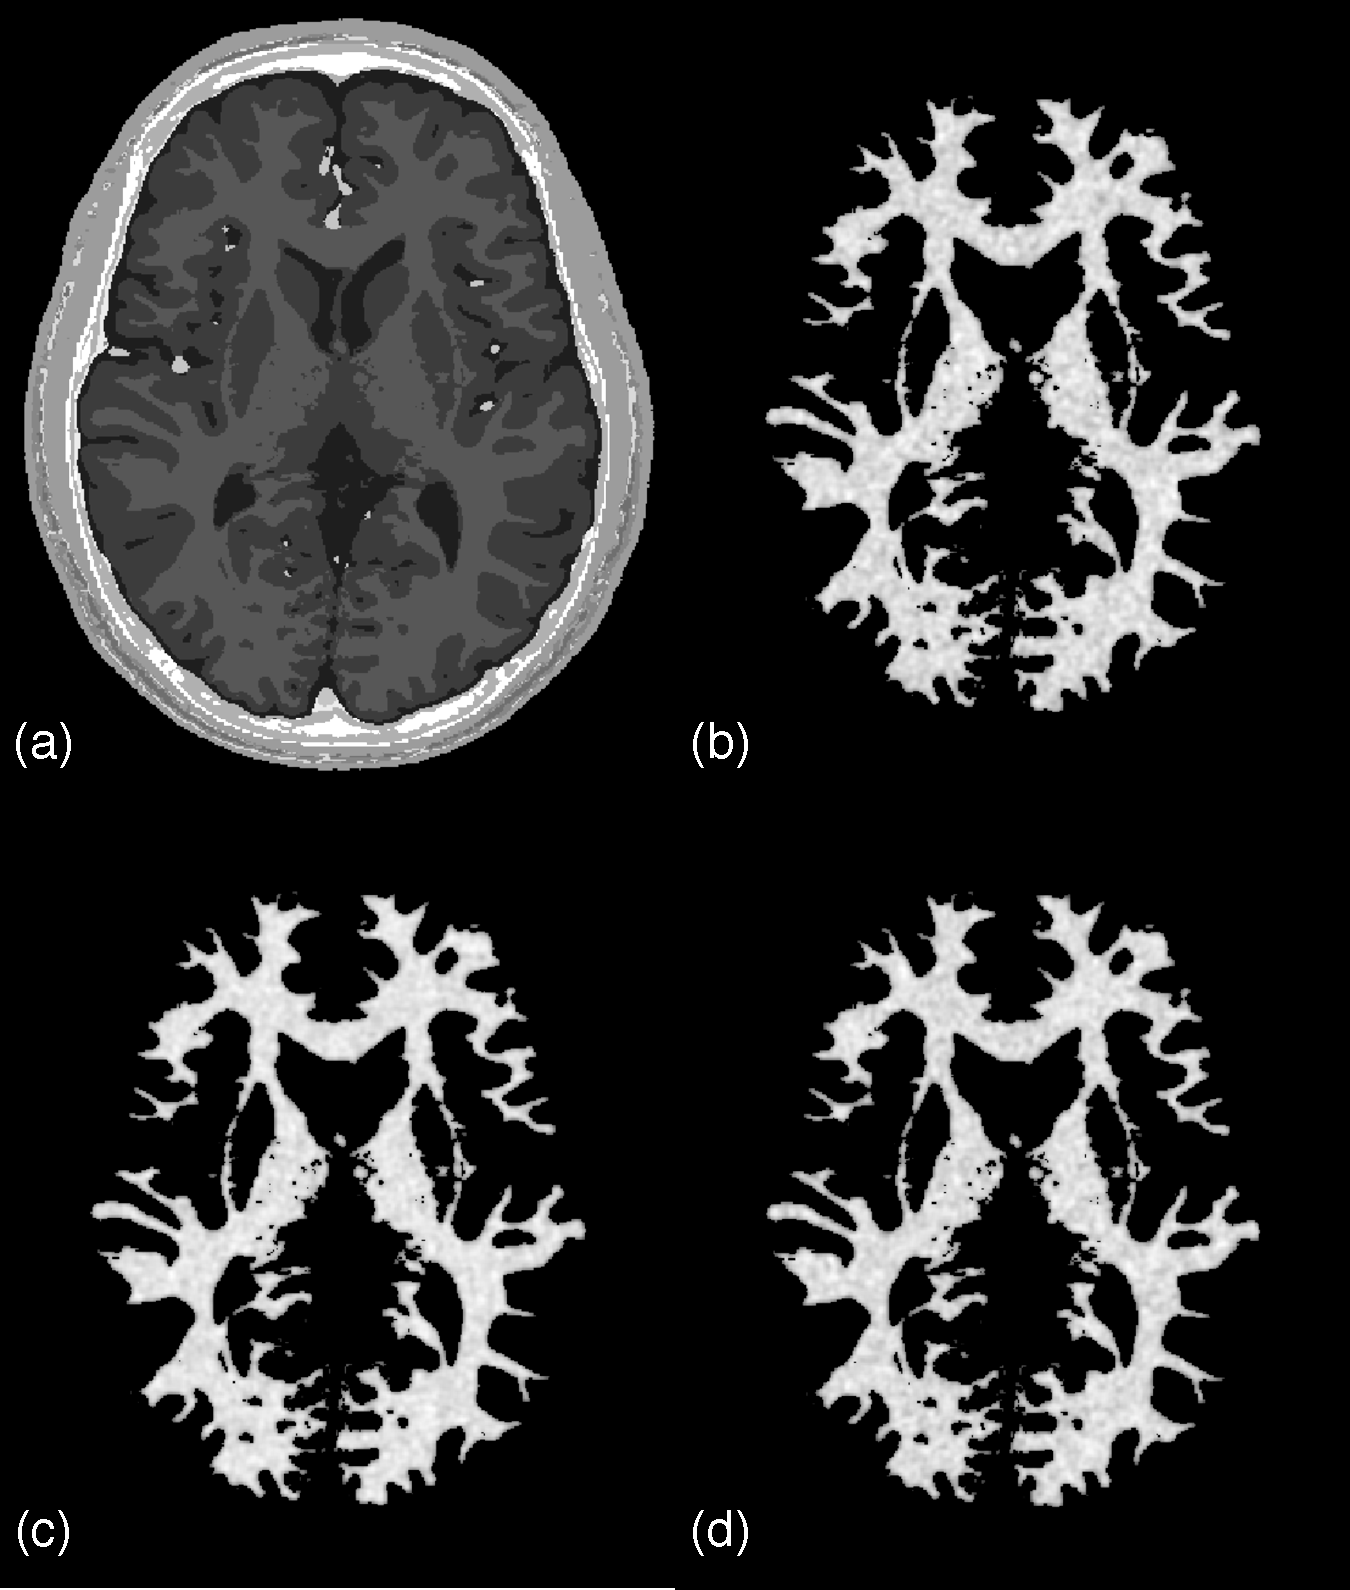
\includegraphics[width=85mm]{simulatedData.jpg}
\end{tabular}
\caption{(a) Axial slice from the discrete BrainWeb data set.  From (a) 
we create the (b) simulated template and sample (c) control and (d) patient images with both 
additive noise and subsequent Gaussian smoothing. }
\label{fig:simulated_data}
\end{figure}

\begin{figure}
\begin{tabular}{c}
  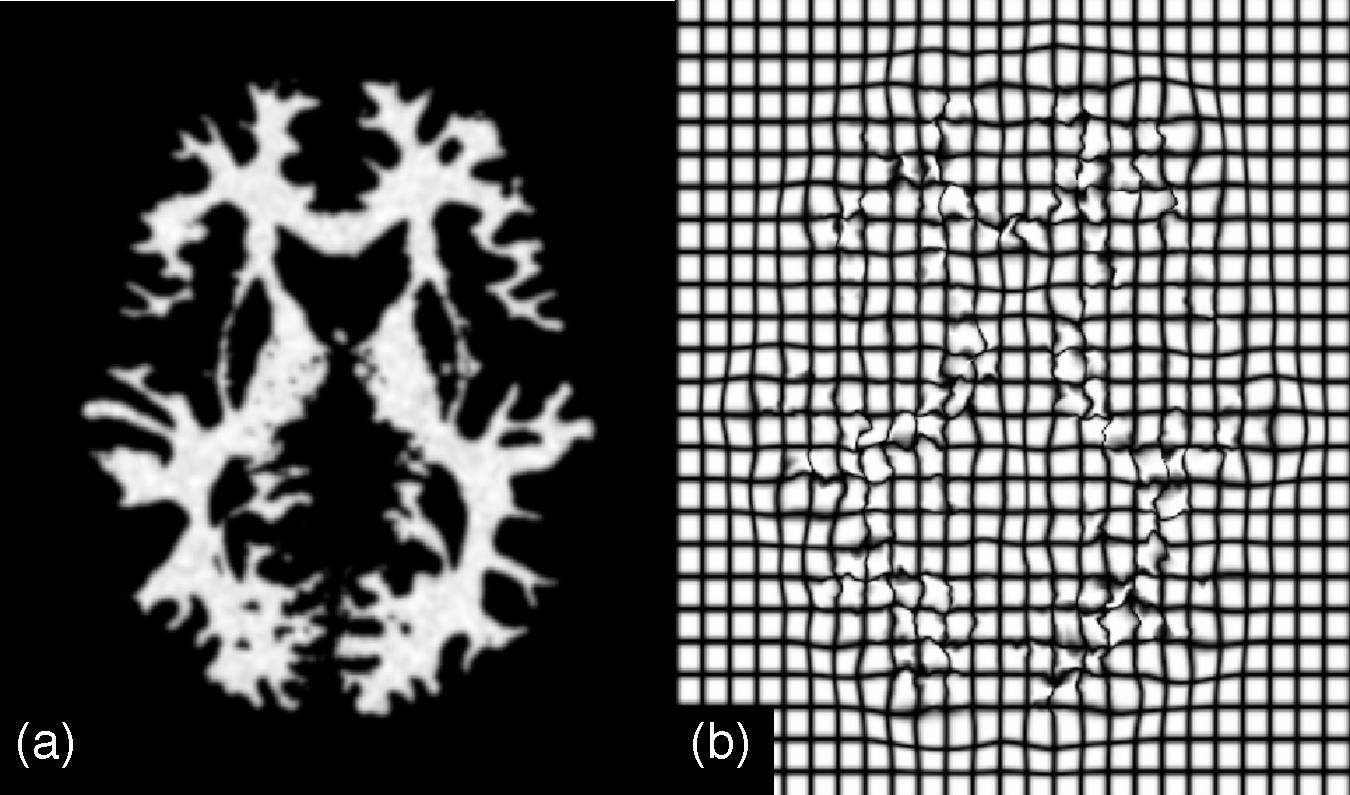
\includegraphics[width=85mm]{simulatedDataWarped.jpg}
\end{tabular}
\caption{Warping the image in Fig. \ref{fig:simulated_data}(c) to the template in 
  Fig. \ref{fig:simulated_data}(b) using the SSD similarity metric produces the image shown in
  (a).  The corresponding deformation is given in (b).  Although the images were anatomically
  aligned prior to invoking ANTs registration, deformation is driven by the similarity metric
  causing the accumulation of type 1 errors.}
\label{fig:simulated_data_warped}
\end{figure}


Axial slice number 159 was extracted from \verb#subject_04# of the discrete BrainWeb database
\cite{Aubert-Broche2006} which is shown in Fig. \ref{fig:simulated_data}.  After thresholding out 
the white matter and assigning all white matter voxels a value of 0.7, 10\% of these white 
matter voxels were randomly selected to be assigned a value of 0.6 in the simulated control 
template and a value of 0.3 in the simulated patient template.  
Note that these values were arbitrarily selected to be more or less in the range of typical
FA values.  Gaussian noise (mean = 0.0, standard deviation = 0.1) was added to the white
matter template followed by a Gaussian smoothing (standard deviation = 1.5 mm) shown in Fig. \ref{fig:simulated_data}(b).  A simulated control cohort was created consisting of 20 subjects.  
Starting with the simulated control template, each of the 20 subjects is created by adding
Gaussian noise (mean = 0.0, standard deviation = 0.1) followed by 
Gaussian smoothing (standard deviation = 1.5 mm).  Thus, each subject is differentiated only by a unique random draw from the noise distribution and there is no real shape difference between subjects.  A simulated patient cohort of 20 subjects
was created similarly using the simulated patient template.  A sample control subject and sample
patient subject are given, respectively, in Fig. \ref{fig:simulated_data}(c) and (d).

\begin{figure*}
\begin{center}
\begin{tabular}{c}
  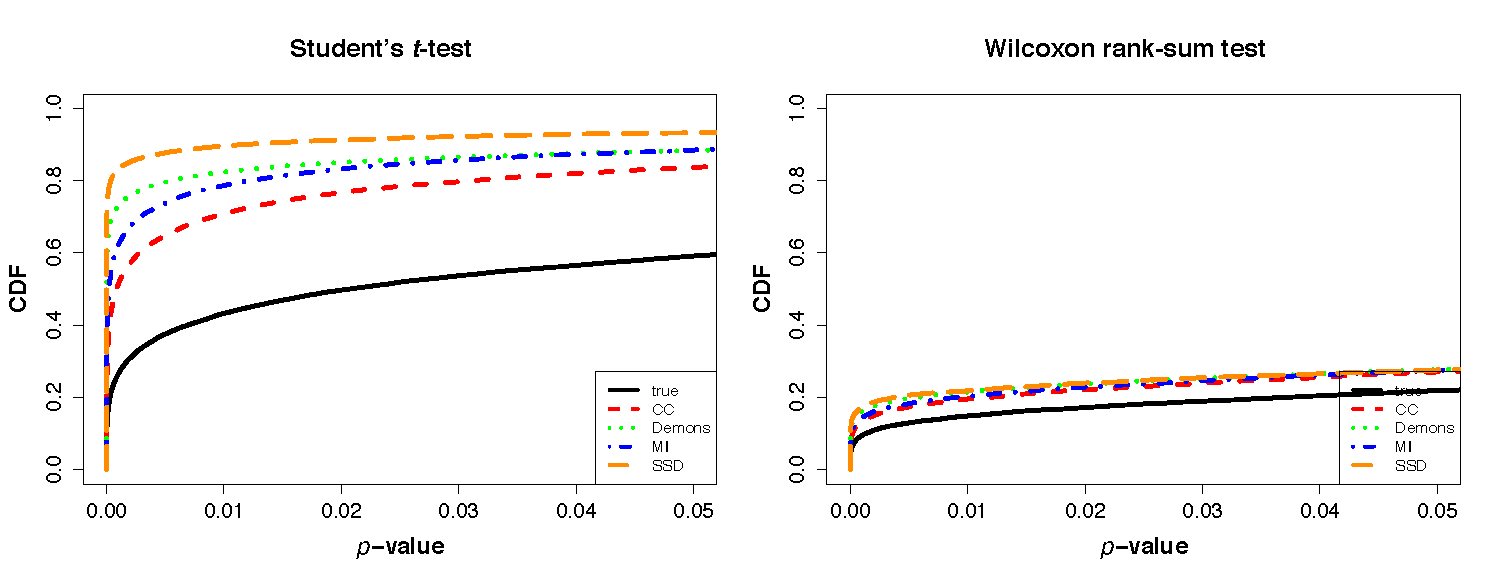
\includegraphics[width=180mm]{simulatedTesting.jpg}
\end{tabular}
\caption{Student's $t$-test and the nonparametric Wilcoxon rank-sum test results (one-tailed, $\alpha = 0.95$) for the simulated experiment adjusted for multiple comparisons (FDR).
The true significance curves are drawn in black.  Elevated statistical power is seen with all 4 
         metrics for both tests although the effect is less in the more robust Wilcoxon results. Not shown are the significance curves for the Brunner-Munzel testing \cite{Rorden2007} which showed similar effects to the results on the left.
        }
\label{fig:simulated_testing}
\end{center}        
\end{figure*}



After creation of the simulated data set, we performed voxelwise testing (both $t$-testing
and Wilcoxon rank-sum testing, one-tailed, $\alpha = 0.95$) with false discovery
rate correction within the white matter to get ``true'' cumulative distribution functions (CDFs).  The CDF vertical axis shows the cumulative number of voxels with corrected $p$-values at or below a given significance level (horizontal axis) and thus may be used as a surrogate measure for spatial sensitivity.  From here, we denote these graphs as "statistical significance curves."  These curves are plotted in black in Fig. \ref{fig:simulated_testing}.  To illustrate the 
effect of similarity metric on statistical significance, we performed ANTs registration \cite{Avants2011} of each subject to the template
(Fig. \ref{fig:simulated_data}(b)) using cross correlation (CC), mutual information (MI), 
Demons \cite{Thirion1998}, and sum of squared differences (SSD). A representative deformed image
using the SSD metric and its corresponding deformed grid is given in 
Fig. \ref{fig:simulated_data_warped}. 
The resulting statistical significance curves are plotted with the true significance curves in Fig. 
\ref{fig:simulated_testing}.  

This example demonstrates the undesirable phenomenon previously described.  Even though these images were anatomically aligned prior to registration, the resulting deformations (falsely) increased detection power.  This effect can be explained in the context of Eqn. (\ref{eq:variance}) and by the fact that we added noise to the underlying distribution which allows the deformable mapping algorithms the freedom to transform the positions of the most "powerful" voxels to minimize variance across the population (and increase the $t$-test).  Note, however, that this effect is increased by the fact that noise was added to the data.  Decreasing the standard deviation of the noise causes an increase in separation between  the SSD and Demon's metric pair with the MI and CC metric pair with the latter pair closer to the the true significance curve. Increasing the noise yields the same ranking with a more even spread between significance curves.

Common similarity metric functions can therefore induce false positives by minimizing local intensity 
variance between the subjects and template which explicitly maximizes statistical
testing results in contrast to maximizing anatomical alignment.  This effect is strongest in 
the SSD and Demons metrics and weakest in the MI and CC metrics likely due
to the degree of correspondence to Eqn. (\ref{eq:variance}).   This is also supported by contrasting
the $t$-test results given in Fig. \ref{fig:simulated_testing}(a) with the non-parametric Wilcoxon
rank-sum testing (Fig. \ref{fig:simulated_testing}(b)).  The rank test does not explicitly use variance in its assessment and thus exhibits far less statistical exaggeration even though it offers roughly 95\%
the power of the $t$-test assuming certain assumptions are met \cite{Siegel1988,Rorden2007}.  

Although various processing choices mitigate these effects, such as Gaussian smoothing, nonparametric testing, and the use of more robust similarity metrics, such choices are often made on an ad hoc basis.  
In contrast, in this work we strongly advocate the general application
%A more principled approach is the use of an anatomical, i.e. T1-weighted, unbiased shape/intensity 
%template constructed from the population images.  DTI-derived scalar images can then be mapped 
%to their corresponding T1-weighted image in a highly constrained manner and subsequently 
%mapped to the template via nonrigid registration of the T1-weighted image.  This minimizes 
%possible complications associated with direct FA-to-FA image registration.
%We recognize that using the anatomical images in the alignment process has been previously proposed (in fact, such a suggestion occurs in the {\it Future directions} section of the original TBSS paper).  
of a high performance \cite{Klein2009}, nonrigid registration algorithm \cite{Avants2011}, which forms the underlying machinery for an optimal template construction algorithm \cite{Avants2010}, in facilitating alignment between DTI-derived scalar images for cross-population studies.  The key point, here, is that the FA images are mapped to the common reference space via intra-subject DT-to-T1 mapping followed by T1-to-T1 alignment.  The T1-to-T1 step is (statistically) independent of the FA values which are the ultimate statistical target of hypothesis testing in FA population studies.  Below, we show that this same pattern of effects is reproduced in real data and detail our proposed solution.  

\begin{figure*}
\begin{center}
\begin{tabular}{c}
  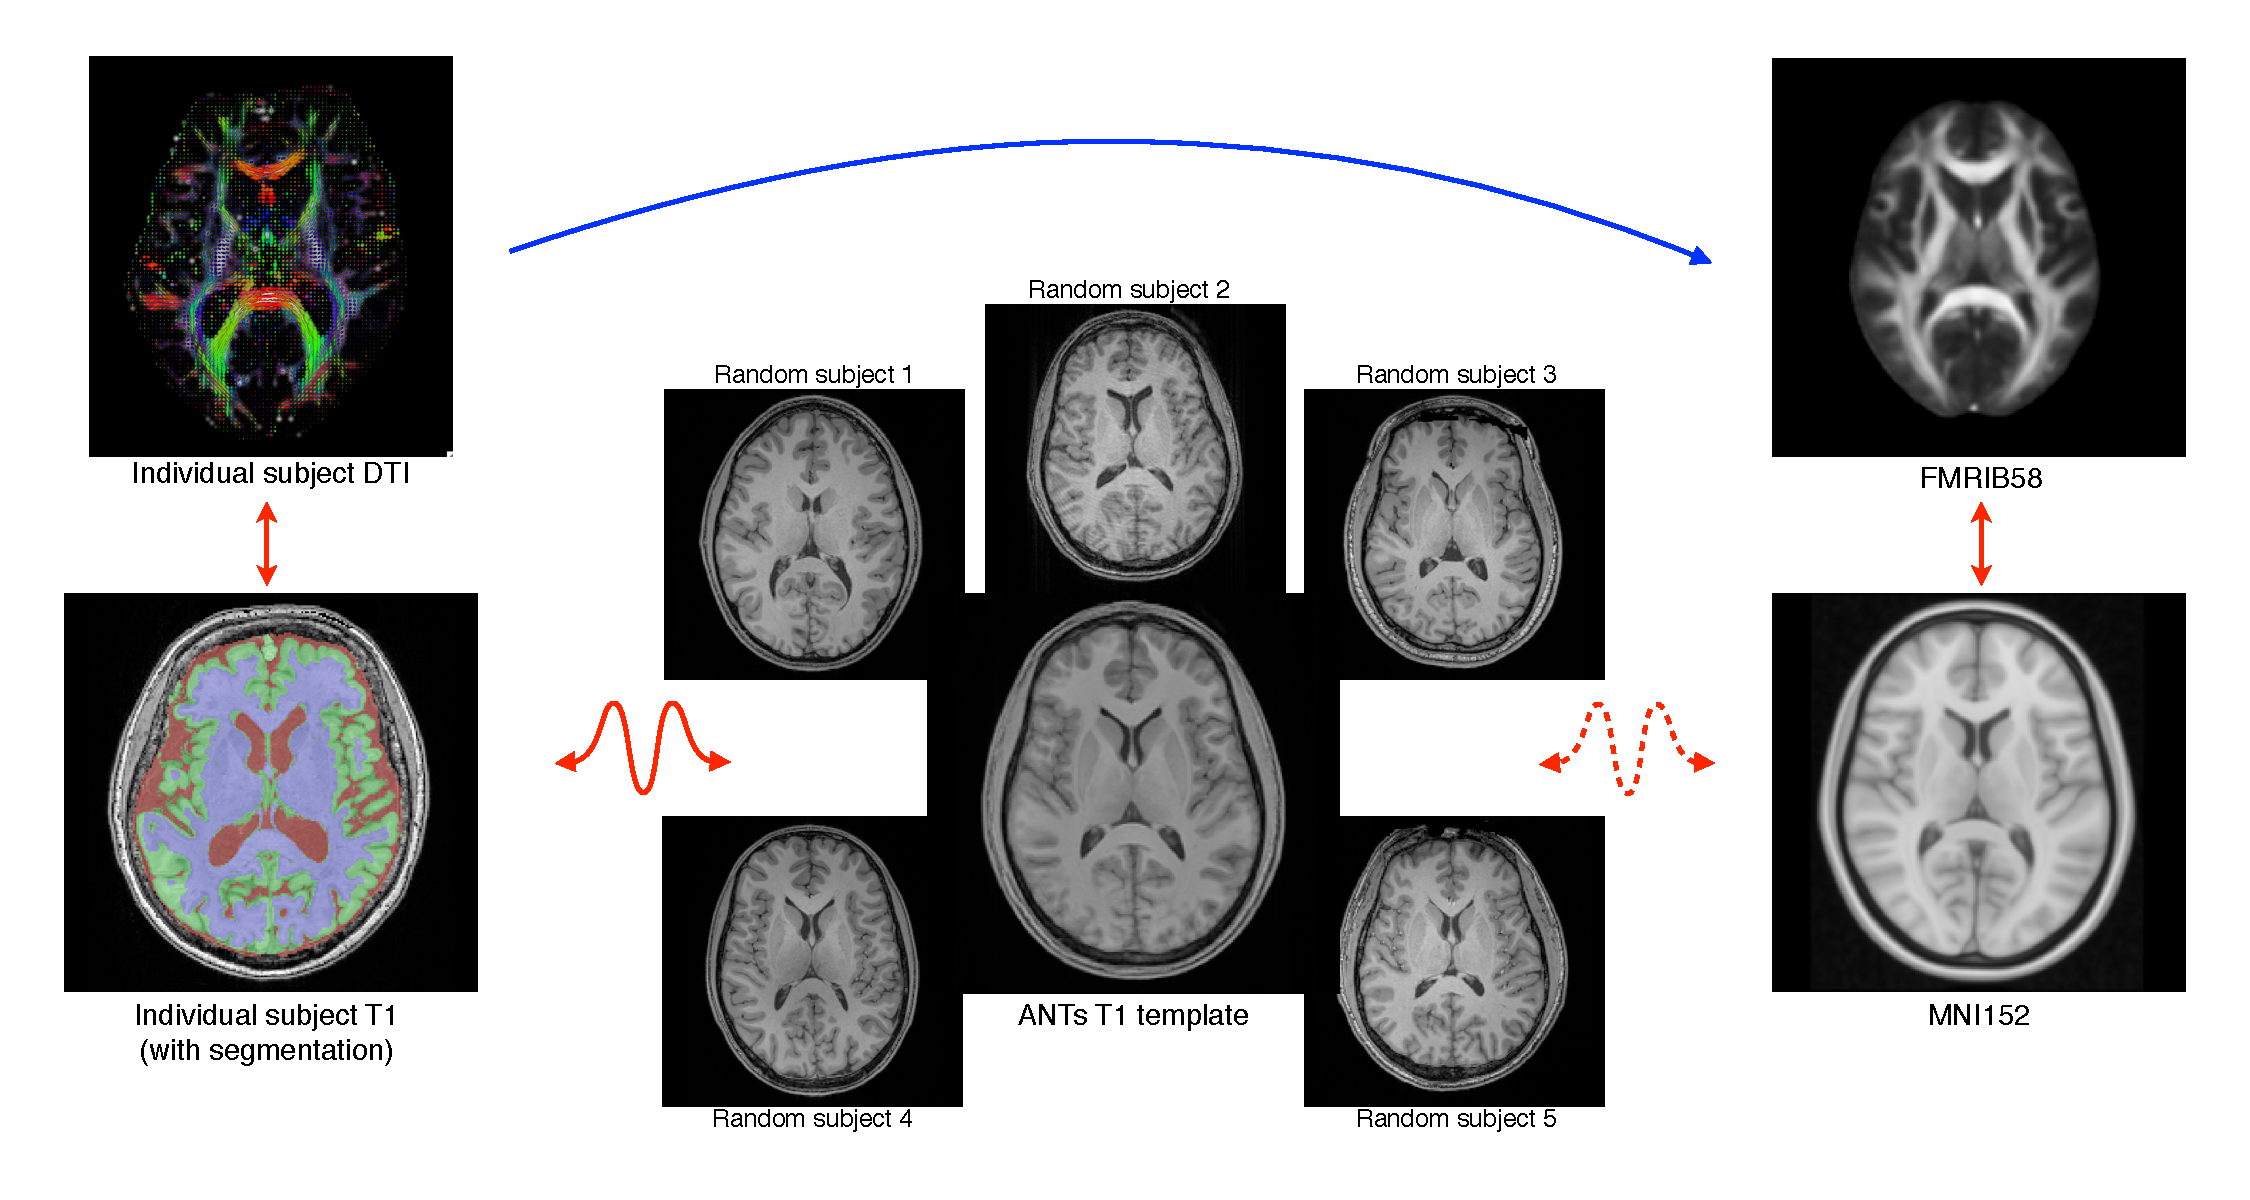
\includegraphics[width=170mm]{workflow.jpg}
\end{tabular}
\caption{Possible ANTs-based TBSS workflow.  In contrast to standard TBSS in which an individual subject's FA is registered to the FMRIB58 template
(transform represented with the blue arrow), our proposed modification first constructs an ANTs optimal anatomical template as illustrated in the center of the figure.  Each FA image is then rigidly mapped, with distortion correction, to the individual T1 using the white matter mask as shown on the left.  The individual T1-weighted image is then nonrigidly registered to the anatomical template.  Optionally, one can register the T1 template to the MNI152 template which resides in the same space as the FMRIB58 template.  Thus, the composite transform, carefully constructed without any FA-to-FA image registration, can take an individual subject's FA map (or other DTI-derived measure) to the desired standardized coordinate system.    }
\label{fig:workflow}
\end{center}
\end{figure*}

We first briefly describe the SyGN algorithm used to create anatomical templates.  
We then explain the the step-by-step process for aligning subject FA images to 
the anatomical template (which is facilitated with the various tools available 
in ANTs).  After describing the real image data used in this work, we show the 
issues raised affect common analysis scenarios.






%
%
%
%It was precisely due to these concerns that the TBSS framework was developed constituting an entire processing pipeline spanning from the reconstruction of the DTI tensorial data
%%to the calculation of the corresponding DTI-derived scalar measures (typically fractional anisotropy (FA)), to the nonrigid alignment of the population to a standard coordinate system and skeletonization, and, finally, 
%through to the statistical analysis for discerning differences across populations.  Major intermediate steps include the calculation of the corresponding DTI-derived scalar measures (typically fractional anisotropy (FA) \cite{Basser1996}), nonrigid alignment of the population to a standard coordinate system, and subsequent ``skeletonization'' of the mean of the aligned FA maps.  The alignment to a standard space is performed in such a way to remove the smoothing step associated with SPM.  Skeletonization and its projection across all registered DTI-derived scalar images is meant to accommodate the possibility of imperfectly aligned data.  However, as shown in a recent study \cite{Zalesky2011}, although the alignment error is reduced with the skeleton projection step, misalignments still remain post-projection.  Added to this is the potential confounding effect of minimizing data differences via nonrigid registration which are potentially the precise differences to be statistically quantified.



%Because spatial normalization is critical to obtaining valid results, we propose a modification of the standard TBSS pipeline directed at some of these residual concerns which we refer to as ANTs-TBSS.  Instead of DTI-derived scalar alignment via the images themselves (either random subject selection or locating an approximation to the ``mean subject'') or to a standard template (e.g. FMRIB58\_FA\_1mm.nii.gz which we denote as ``FMRIB58'' in the remainder of the text), we evaluate the substitution of an anatomical, i.e. T1-weighted, unbiased shape/intensity template constructed from the population images.  DTI-derived images can then be mapped to their corresponding T1-weighted image in a highly constrained manner and subsequently mapped to the template via nonrigid registration of the T1-weighted image.  This eliminates any possible complications associated with direct FA-to-FA image registration.







%We first describe in greater detail the proposed ANTs-TBSS framework with an emphasis on comparison with standard TBSS.  We then describe the two open data sets used to evaluate the proposed methodology in addition to a description of diffuse TBI data 
%also used to illustrate concepts discussed in this work.
%and analysis previously reported in \cite{Avants2008}.   
%The complementary assessment performed in this paper is used to provide additional analyses to these previous findings.

%A crucial component of TBSS is the alignment of the DTI-derived scalar images \cite{Zalesky2011}. 
%
%Voxel-based morphometry vs. tractography vs. tract-specific analysis
%
%Talk about {\em skeleton projection} and how our work is different from \cite{Zalesky2011}.
%Also talk about the advantages over building a dti-based template as discussed in 
%\cite{Hecke2010}.



\section{Material and Methods}

%Provide sufficient detail to allow the work to be reproduced. Methods already published should be indicated by a reference: only relevant modifications should be described.

%In order to understand the differences in approaches, we first briefly describe
%the current TBSS protocol as it is implemented.  This is followed by a
%brief outline of the proposed modification using ANTs.  Afterwards
%we give a description of the data sets used to demonstrate the methods.


\subsection{Anatomical Image Template Construction}
In general, we normalize images to to a standard coordinate system to
reduce intersubject variability in population studies.  Various
approaches exist for determining the normalized space such as selection
of a pre-existing template based on a single subject, e.g. the Talairach
atlas \cite{Talairach1988}), or a publicly available averaged group of
subjects, e.g. the MNI \cite{Collins1994} or ICBM \cite{Mazziotta1995}
templates.  One challenge with standard templates is that they may inadvertantly bias one's results by enabling better normalization of subjects to which the template is more similar.  This issue is exacerbated when dealing with populations that have high variance (e.g. due to disease) and/or when one's normalization method is low-dimensional (not flexible enough to capture large shape differences). 

Population-specific templates (or optimal templates) alleviate some of
these issues by deriving a most representative image from the population
\cite{Good2001}.  Large deformation registration algorithms also reduce
this confound by being less sensitive to the deformation distance
between subject and target.  Some approaches combine both advantages,
for instance, the diffeomorphic approach of Joshi et al. who employ the
SSD metric and a shape distance to bring the subject group of images
into alignment \cite{Joshi2004}.  Variants
include extension to multiple modalities \cite{Lorenzen2006} and small deformations
\cite{Geng2009}.  These approaches iteratively minimize group difference in ``congealing''
towards a representative image template \cite{Learned-Miller2006}.

In contrast, Avants et al. explicitly model the geometric component of the 
normalized space during optimization.  Coupling the intrinsic symmetry of 
SyN pairwise registration \cite{Avants2011} and an
optimized sharpening/averaging of the template appearance, Symmetric Group
Normalization (SyGN) is a powerful framework for producing optimal population-specific
templates \cite{Avants2010} with arbitrary similarity metric choice. Given a set of representative images, 
$\{I_1, I_2, \ldots, I_M\}$, optimization involves finding the set of paired
diffeomorphic transformations, $\left\{\left(\phi^1_1, \phi^1_2\right), 
\left(\phi^2_1, \phi^2_2\right), \ldots, \left(\phi^M_1, \phi^M_2\right) \right\}$,
the optimal template appearance, $J^*$, and corresponding coordinate system, $\psi(\mathbf{x})$,
which minimize the following cost function:
\begin{align}
  \sum_{m=1}^M \left[
    D\left( \psi(\mathbf{x}), \phi^m_1(\mathbf{x}, 1) \right) + 
    \Pi \left( I_m\left(\phi^m_2(\mathbf{x}, 0.5) \right), J^*\left(\phi^m_1(\mathbf{x}, 0.5) \right) \right)
    \right]
\end{align}
where $D$ is the diffeomorphic shape distance, 
\begin{align}
  D\left(\phi(\mathbf{x}, 0), \phi(\mathbf{x}, 1)\right) = \int_{0}^1 \| v(\mathbf{x}, t) \|_L dt, 
\end{align}
dependent upon the choice of the linear operator, $L$, and
$v$ is the diffeomorphism-generating velocity field, 
\begin{align}
  v\left(\phi(\mathbf{x}, t), t \right) = \frac{d\phi(\mathbf{x}, t)}{dt},\,\,\, \phi(\mathbf{x}, 0) = \mathbf{x}.
\end{align}
$\Pi$ is the choice of similarity metric, often cross-correlation \cite{Avants2008a}, calculated in the 
virtual domain midway between each individual image and the current estimate of the template. 

With initial assignment of $\left\{\left(\phi^m_1, \phi^m_2\right)\right\}$ and $\psi(\mathbf{x})$ 
to identity, iterative optimization
involves estimating the pairwise transformations, estimation of the optimal template appearance, and 
updating $\psi(\mathbf{x})$ by averaging the current estimate of $\left\{\phi_1^m\right\}$.  Additional details are given in \cite{Avants2010}.  
%For the interested reader, a set of scripts has been created and is distributed with the ANTs library for facilitating template creation.


\subsection{Anatomically-Based Population Normalization}
We now detail a standard approach that uses SyGN and intra-subject inter-modality mapping to provide an unbiased strategy for FA normalization.
An example of our proposed workflow applied to anatomically-based population normalization prior to FA analysis is illustrated in Fig. \ref{fig:workflow}.  Instead of direct FA-to-FA registration, our ANTs-based modification can be described as follows:

\begin{enumerate}
  \item Build the anatomical template from  the population sample or sample subset using SyGN as described in
  the previous section.
  \item If only using a sample subset for template creation, register the remaining
        anatomical data to the template and save the resulting transformation for each         
        subject indexed by $i$ (i.e. $\mathcal{T}^i_{template}$).
  \item Find the optimal transformation from each
        subject's FA to the anatomical template:
  \begin{enumerate}
  \item For each anatomical image, segment the white matter (in ANTs, one can use N4 bias correction \cite{Tustison2010} and Atropos $n$-tissue segmentation \cite{Avants2011a}).
  \item Rigidly transform each subject's average DWI to the bias-corrected anatomical image ($\mathcal{R}^i_{dwi}$).
  \item Perform distortion correction on the FA to anatomical mapping 
        by localized nonrigid registration
        of rigidly transformed FA map ($=\mathcal{R}^i_{dwi} \mathrm{FA}$) using
        the white matter mask obtained in step 3(a) ($\mathcal{T}^i_{FA}$).
  \item For each subject, concatenate the transforms which maps each
        subject's FA to the template ($\mathcal{T}^i_{total} = \mathcal{T}^i_{template} \circ 
        \mathcal{T}^i_{FA} \circ \mathcal{R}^i_{dwi} \mathrm{FA}$).
  \item Warp each subject's FA map to the template using $\mathcal{T}^i_{total}$.  Equivalently, one could warp the mean diffusion (MD), axial diffusion (AD) or any other scalar derivable from DTI to the template.  One other detail is that we prefer to warp the subject's DTI to the template and then, in template space, derive the scalar images of interest.  
  \end{enumerate}      
%  \item Perform the remaining portions of the standard TBSS pipeline:
%    \begin{enumerate}
%      \item Create the mean FA image from all template-aligned FA images.
%      \item Produce the white matter skeleton from the mean FA image.
%      \item Create skeleton distance map and project all FA data onto the skeleton.
%      \item Run the statistical analysis.
%    \end{enumerate}
\end{enumerate}
The next section compares this framework to FA-based normalization strategies with respect to both a patient-control study and a study of gender and age effects in a control population.  

\subsection{Imaging Data}
Diffusion tensor data associated with each of the following data sets were reconstructed from the diffusion weighted sequences using Camino%
\footnote{
http://camino.org.uk/
}---an open source toolkit for diffusion MRI processing and analysis \cite{Cook2006} in combination with ANTs-based registration for motion correction of the DTI sequence.

\subsubsection{Diffuse Traumatic Brain Injury Data}

The TBI data used in this study is part of a larger effort investigating the relationship between various neuroimaging indices and cognitive and functional abilities in long-term survivors of TBI (principal investigator: John Whyte). A more detailed data description can be found in \cite{Avants2008}. The following is a brief description relevant to our particular study.  
17 controls and 16 patients with TBI were used for the analysis presented in this work.  Each patient had a history of non-penetrating traumatic brain injury 
of at least moderate severity defined by significant and well-documented
loss or alteration of consciousness following injury in addition to meeting
several other exclusionary criteria.  The healthy volunteers were matched in terms of age, gender, ethnicity, handedness, and years of education.
High resolution T1-weighted anatomic images were obtained using a 3D MP-RAGE 
imaging sequence with the following acquisition parameters: TR = 1620 ms, 
TI = 950 ms, TE = 3 ms, flip angle = 15$^\circ$, 160 contiguous slices of 
1.0 mm thickness, FOV = 192 $\times$ 256 mm$^2$, matrix = 192 $\times$ 256, 
1NEX with a scan time of 6 minutes, and voxel size = 1 mm$^3$.  30-directional
DTI images were also obtained. 
%
%\subsubsection{Participants}
%{\color{red}{Quote:}} The data were collected as part of a larger study investigating the neural correlates of attention deficits and treatment responses of various psychoactive drugs in the survivors of TBI (principal investigator: J.W.). Thirty individuals with TBI and 20 healthy volunteers were recruited. We planned to recruit more TBI participants because data of TBI survivors are more likely to be discarded in a typical functional neuroimaging study due to movements in the scanner and poor behavioral performance. TBI participants were recruited from a variety of clinical services at MossRehab and through a consent-based registry of individuals with TBI who are interested in participating in rehabilitation research. To be included, participants had to be between the ages of 16 and 60, and to have a history of non-penetrating traumatic brain injury of at least moderate severity at least 3 months prior to enrollment. Severity level was defined by significant and well-documented loss or alteration of consciousness following injury (i.e., lowest Glasgow Coma Scale (GCS) score of less than 12, or prospectively documented post-traumatic amnesia (PTA) of greater than 1 hour), or focal abnormality on a neuroimaging study that was attributable to traumatic injury. A subjective complaint of attention difficulties by the participant, treating clinician, or caregiver was also required. Potential participants were excluded if they had a history of prem orbid neurologic disease, psychosis, major affective disorder, mental retardation, Attention Deficit Hyperactivity Disorder, or if they were currently abusing alcohol or recreational drugs. Persons who were taking psychoactive medications other than anticonvulsants were also excluded. Participants and/or their involved caregivers (depending on the participant�s cognitive capacity) provided informed consent. The study protocol was approved by the Albert Einstein Healthcare Network and the University of Pennsylvania IRBs. Twenty healthy volunteers, matched to patients for age, gender, handedness, years of education, and ethnicity, participated in the study. Control participants were recruited based on the same inclusion/exclusion criteria as patients, with the exception that they never had a TBI resulting in loss or alteration of consciousness, nor suffered attention complaints. Control participants were recruited through the family and friendship networks of the participants with TBI, and through public advertising.
%Data from one TBI participant whose MRI scan showed a large area of encephalom alacia over almost the entire right hemisphere were excluded. The remaining 29 subjects with TBI included 21 men and 8 women aged between 18 and 58 years (mean age = 36.9, SD = 11.4) with a mean education of 13.1 years (SD = 2.8). Twenty three of them were right-handed (Edinburgh Handedness Inventory, Oldfield, 1971). Fourteen of them were Caucasians, 10 African Americans, 4 Hispanics, and 1 Asian. Selected demographic and clinical characteristics of the TBI survivors are reported in Table 1. Control participants included 17 men and 3 women aged between 21 and 50 years (mean age = 34.9, SD = 9.8) with a mean education of 13.1 years (SD = 1.7). Sixteen of them were right-handed. Eleven of them were Caucasians, 7 African Americans, 1 Asian, and 1 unknown. The two groups did not differ significantly in terms of age, gender, ethnicity, handedness or years of education (tested with t-test or Fisher�s exact test, as appropriate).
%
%\subsubsection{Image acquisition}
%The functional imaging was conducted on a Siemens 3.0 T Trio whole-body scanner (Siemens AG, Erlangen, Germany), using a standard Transmit/Receive head coil. High resolution T1-weighted anatomic images were obtained using 3D M PRAGE imaging sequence using the following acquisition parameters: TR = 1620 ms, TI = 950 ms, TE = 3 ms, flip angle = 15$^\circ$, 160 contiguous slices of 1.0 mm thickness, FOV = 192 $\times$ 256 mm$^2$, matrix = 192 $\times$ 256, 1NEX with a scan time of 6 minutes. The resulting voxel size was 1 mm$^3$.
%Lesion assessment
%To quantify the volume of lesions, a trained observer (J.P.) manually segmented the lesion area under supervision of a neurologist (H.B.C.) with extensive experience in lesion assessment. Focal lesions included any cystic cavities and other focal regions of abnormal signal in the white or gray matter. The ITK-SNAP software \citep{Yushkevich2006} was used for a 3D-based segmentation. Total lesion volume was calculated using a stand-alone utility provided by VoxBo software (Center for Functional Neuroimaging, Philadelphia, PA, http://www.voxbo.org).





\subsubsection{Data from the International Neuroimaging Data-sharing Initiative (INDI)}

In support of open science, the 1000 Functional Connectomes Project (FCP)%
\footnote{
ttp://fcon\_1000.projects.nitrc.org
} 
was initiated on December 11, 2009 by various members of the MRI community \cite{Biswal2010}.  Motivated by the absence of neuroimaging data for research, this initiative seeks to form collaborative partnerships with imaging institutions for sharing well-documented multi-modal image sets accompanied by phenotypic data.
Commitments from institutions such as they NYU Institute for Pediatric Neuroscience and the Nathan Kline Institute (NKI)--Rockland have already resulted in prospective data repositories
currently distributed to the public via the Neuroimaging Informatics Tools and Resources Clearinghouse (NITRC).%
\footnote{
http://www.nitrc.org
}
%Data from these two institutions were used to demonstrate the alignment properties obtained using SyGN for DTI-derived data normalization.

\paragraph{NKI/Rockland Sample}
Data from the first 14 weeks of prospective data-sharing were downloaded on January 15, 2011 comprised of 74 subjects (average age in years: 32.4 $\pm$ 17.8).  
Due to various issues (e.g. lack of corresponding T1 image, failed DTI reconstruction, and age matching requirements) only 57 subjects were used for the first alignment analysis and 27 subjects of the NKI data set were used for the second analysis consisting of 9 females (age: $29.3 \pm 6.6$ years) and 18 males (age: $ 26.6 \pm 6.9$ years).
Germane to our evaluation, each imaging session for each subject produced a 64-directional diffusion tensor imaging scan (parameters: conventional single-shot spin echo
EPI pulse sequence, TR = 10000 ms, TE = 91 ms, axial acquisition, 
voxel size = $2 \times 2 \times 2$ mm$^3$) and a T1 anatomical scan (parameters:  TR = 2500 ms, b = 1000 s/mm$^2$ for each direction, 58 contiguous slices of 2.0 mm thickness,
TI = 1200 ms, TE = 3.5 ms, flip angle = 8$^\circ$, 192 contiguous slices of 
1.0 mm thickness, FOV = 256 $\times$ 256 mm$^2$, and voxel size = 1 mm$^3$).  Images were anonymized including defacing of the T1 images prior to upload. 


%\paragraph{NYU Institute for Pediatric Neuroscience Sample}
%Data from the first 3 parts of prospective data-sharing from NYU were also downloaded on January 15, 2011 comprised of 49 subjects (average age in years: 30.29 $\pm$ 8.81).  All subjects were used in the image alignment assessment.  Two 64-directional DTI scans were performed (parameters: conventional single-shot spin echo
%EPI pulse sequence, TR = 5200 ms, TE = 78 ms, axial acquisition, 
%voxel size = $3 \times 3 \times 3$ mm$^3$) and a T1 anatomical scan (parameters:  TR = 2530 ms, TE = 3.25 ms, flip angle = 7$^\circ$, 256 contiguous slices of 1.33 mm, FOV = 256 $\times$ 256 mm$^2$, and voxel size = 1.3 mm$^3$).  Images were anonymized including defacing of the T1 images prior to upload. 

%
%The 1000 Functional Connectomes Project (FCP)%
%\footnote{
%http://fcon\_1000.projects.nitrc.org/index.html
%}
%
%{\color{red}{Quote}}  INDI is a next-generation data-sharing effort, with the goal of sharing phenotypically rich imaging datasets, on both retrospective and prospective bases. On 10/8/10, the Nathan Kline Institute (NKI) / Rockland Sample led the way for INDI-Prospective, starting weekly uploads of 5-7 subjects / week (R-fMRI, DTI, and extensive psychiatric and cognitive phenotypic data, including IQ), which continue to progress (currently n = 55 and growing!). More recently, the NYU Institute Pediatric Neuroscience released its sample examining cocaine dependence in adults via INDI-Retro. The list of sites pledging data from around the world is growing, and we are working to generate common phenotypic variables across datasets as possible (notice the frequency with which IQ is starting to appear � it�s just one of our targets!). 
%
%\subsubsection{Nathan Kline Institute (NKI) / Rockland Sample}
%
%{\color{red}{Quote}}  The NKI/Rockland Sample is intended to be a phenotypically rich neuroimaging sample, consisting of data obtained from individuals between the ages of 6 and 85 year-old. All individuals to be included in the sample undergo semi-structured diagnostic psychiatric interviews, and complete a battery of psychiatric, cognitive and behavioral assessments in order to provide comprehensive phenotypic information for the purpose of exploring brain/behavior relationships.
%
%Each subject consists of the following data:
%\begin{itemize}
%\item 10 minute resting state fMRI scan (R-fMRI) 
%\item 6-direction diffusion tensor imaging (DTI) scan 
%\item 64-direction diffusion tensor imaging scan (2mm isotropic)
%\item MPRAGE anatomical scan
%\item A variety of psychiatric, cognitive and behavioral assessments
%\end{itemize}
%
%\subsubsection{NYU Institute for Pediatric Neuroscience}
%
%{\color{red}{Quote}}  Summary: The NYU Phyllis Green and Randolph C?wen Institute for Pediatric Neuroscience (IPN) sample will be a collection of past and present scans obtained from psychiatrically screened individuals ranging in age from 6 to 55 years old. The initial release consists of datasets from 49 psychiatrically neurotypical adults, with age, gender and intelligence quotient (IQ) information provided. Future releases will include more comprehensive phenotypic information, and child and adolescent datasets, as well as individuals from clinical populations.
%
%Each subject consists of the following data:
%\begin{itemize}
%\item At least one 6-minute resting state fMRI scan (R-fMRI)%
%\footnote{
% Most participants have 2 R-fMRI scans, collected less than 1 hour apart in the same scanning session. Rest$_1$ is always collected first.
%}
%\item One high-resolution T1-weighted mprage, defaced to protect patient confidentiality
%\item Two 64-direction diffusion tensor imaging scans
%\item Demographic information (age, gender) and IQ-measures (Verbal, Performance, and Composite; Weschler Abbreviated Scale of Intelligence [WASI])
%\end{itemize}
%



\subsection{FMRIB Software Library (FSL)}

FSL hosts a large number of algorithms for computational neuroanalysis.  These include, among others, well-known tools for image segmentation (FAST---\cite{Zhang2001}), linear (FLIRT---\citep{Jenkinson2001}) and nonlinear (FNIRT) image registration, brain extraction (BET---\citep{Smith2002}), and TBSS and made publicly available by the Oxford Centre for Functional MRI of the Brain (FMRIB).
Based solely on the number of citations in the literature,%
\footnote{
As of the beginning of the year 2011, the original Neuroimage 2006 TBSS paper has been cited more than 360 times making it the most cited in the journal's library.
}
usage of TBSS has become a de facto quantitative tool for DTI analysis based, at least in part, on its accessibility and ease of use.  Due to its large presence in the neuroimaging community, many of the comparisons that are performed in the next section use the FMRIB58 template (shown in the upper left of Figure \ref{fig:workflow}).  This template serves as the final coordinate system for most of the comparisons whether it be based on direct normalization or T1 normalization to the MNI152 template which resides in the FMRIB58 space.  We also used the normalization component of TBSS composed of FLIRT and FNIRT registration steps optimized for normalization to FMRIB58 to provide an external comparative baseline (which we denote in subsequent sections as ``tbss'').

%For the comparative evaluation studies used in this manuscript, TBSSv1.2%
%\footnote{
%Build 416 downloaded from the FMRIB web site http://www.fmrib.ox.ac.uk/fsldownloads/ on November 18, 2010.
%}
%was used.  The actual code pipeline constituting TBSS prior to statistical analysis consists of the following 4 shell scripts:
%\begin{description}
%  \item[tbss\_1\_preproc]  Input is a directory of FA images which are slightly eroded and then organized into a separate FA directory.  A mask is also generated for each input FA image for use during the spatial normalization process.
%  \item[tbss\_2\_reg]  The organized FA data and corresponding masks produced in the previous step are warped to one of three possible coordinate systems using FLIRT/ FNIRT:  1)  the atlas included with the FSL download---FMRIB58---(recommended), 2) a user-specified target image or 3) an exhaustive search for the ``optimal'' target image.  In \cite{Smith2006}, page 1491 section {\it Identifying the target for alignment}, the latter option was advocated based on the observation that average FA images tend to be blurred in contrast to the FA of a single subject.  However, even though it would be faster to simply choose a single subject at random, the complexities of nonrigid image registration would seemingly promote the exhaustive search over random selection.   As a compromise between these two options, the first option in the script is to use FMRIB58 which also resides in the space of the MNI152 T1 template.  It should also be noted that this particular script invokes another FSL script, {\bf fsl\_reg}.  An option associated with {\bf fsl\_reg} permits the use of an FNIRT configuration file which has been optimized for use with the FMRIB58 atlas.  
%  \item[tbss\_3\_postreg] The mean FA image is generated from the aligned FA images which is subsequently skeletonized.
%  \item[tbss\_4\_prestats] The skeleton mask is created by thresholding the mean FA skeleton.  The skeleton distance map is then generated and all FA data are projected onto the skeleton.
%\end{description}


\section{Results and Discussion}
%Results should be clear and concise.



\subsection{TBI Cohort} 


\begin{figure*}
\begin{center}
\begin{tabular}{c}
  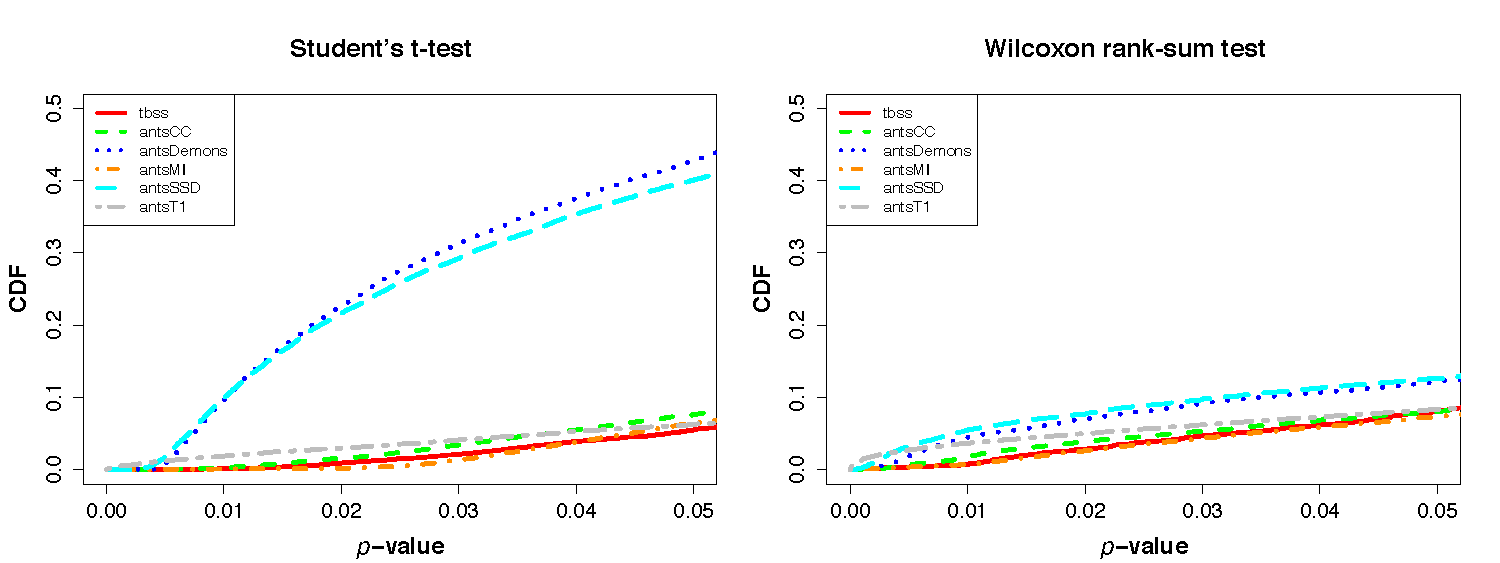
\includegraphics[width=180mm]{tbiTesting.jpg}
\end{tabular}
\caption{Student's $t$-test and the nonparametric Wilcoxon rank-sum test results (one-tailed, $\alpha = 0.95$) for the TBI FA data aligned to the FMRIB58 template adjusted for multiple comparisons (FDR).  Elevated statistical power is seen in the $t$-test with the similarity metrics with the most correspondence to Eqn. (\ref{eq:variance}), namely the SSD and Demons metric which shrinks drastically for the Wilcoxon rank-sum test.  Results for the other metrics including TBSS and the T1 template-based strategy (``antsT1'') remain fairly stable between the two tests.    TBSS and the 4 ANTs metric
results were all obtained using direct registration involving subject FA and the FMRIB58 template.  The antsT1 results were also obtained in FMRIB58 space but the following transformation composition: subject FA $\rightarrow$ subject T1 $\rightarrow$ group T1 template $\rightarrow$ 
common T1 template $\rightarrow$ MNI152 (FMRIB58) template.    }
\label{fig:tbi_testing}
\end{center}        
\end{figure*}


We constructed a patient template and a control template from the T1-weighted images of the two groups.  These two 
templates were then used to create a third common template.  
To compare with TBSS normalization, the common template was
registered to the MNI152 template.  Thus, the transformation
which takes the FA image of an individual subject to the FMRIB58
template is the composition of transforms: 
subject FA $\rightarrow$ subject T1 $\rightarrow$ group T1 template $\rightarrow$ 
common T1 template $\rightarrow$ MNI152 (FMRIB58) template.
We evaluated this strategy relative to direct FA-to-FA
ANTs registration with the common similarity metrics used in
the simulated data example described earlier.
Standard TBSS alignment was also performed.  

Cumulative distribution functions (one-tailed, $\alpha = 0.95$)
are shown in Fig. \ref{fig:tbi_testing}.
Similar to previous findings with the simulated data, the SSD and 
Demons metric show elevated statistical power using the Student's 
$t$-test over the other alignment protocols which all exhibit similar 
strength.  However, this discrepancy decreases significantly with the 
nonparametric testing.  The Demons and SSD power decreases while the others
remain fairly similar.  Interestingly, the ANTs template-based approach
trends towards better performance relative to the remaining 3 strategies.
It should be noted that although TBSS uses the SSD metric, the fixed and moving images are smoothed and subsampled even at the highest resolution level which substantially decreases the local effect of the metric.

\begin{table}
  \caption{Overlap measures of thresholded mean FA and MNI152 white matter.}
  \label{table:lom}
  \begin{tabular*}{88mm}{@{\extracolsep{\fill}} cccccc}
  \hline
%  {} & \multicolumn{2}{c}{NKI} & \multicolumn{2}{c}{NYU} \\
%  \cline{2-5}
  {Norm.} & Target & Jaccard & Dice  & False $-$ & False $+$\\
  \hline
  \hline
  antsT1 & 0.917 & 0.621 & 0.767 & 0.082 & 0.341 \\
  antsCC & 0.780 & 0.570 & 0.727 & 0.220 & 0.320 \\
  antsMI & 0.776 & 0.569 & 0.725 & 0.223 & 0.320 \\
  antsDemons & 0.780 & 0.566 & 0.723 & 0.220 & 0.326 \\
  antsSSD & 0.783 & 0.562 & 0.720 &  0.217 & 0.334 \\
  tbss & 0.716 & 0.550 & 0.710 & 0.283 & 0.295 \\
  \hline
  \end{tabular*}
\end{table} 

The CDF of the voxelwise FA coefficient of variation of the aligned
images is shown for each case in Figure \ref{fig:tbi_cov}.  
The coefficient of variation at each voxel is defined as the variance
divided by the mean over the population of FA values.  Thus,
those metrics which best minimize the voxelwise variance would
trend towards greater alignment as quantified by the coefficient of
variation.

%This is very much related to earlier findings in that strategies evincing
%greater alignment, as quantified by the coefficient of variation,
%will trend towards smaller variance thus exhibiting a left-shifted
%CDF.  

Although direct FA-to-FA registration using ANTs with common
similarity metrics gives ``better alignment'' such alignment is 
produced at a cost of significant type 1 errors.  Common subsampling and
smoothing strategies and local neighborhood metrics such as CC and MI reduce the 
Type 1 error problem (as evidenced in Fig. \ref{fig:tbi_testing}) 
but also show a decrease in alignment.  This is further supported
by the overlap measures \cite{Crum2006} given in Table \ref{table:lom}.
For each alignment strategy, we thresholded the derived mean FA image (FA $
\geq$ 0.2) and compared it with white matter mask of the MNI152 template
segmented using Atropos \cite{Avants2011a}.  The template-based
strategy showed the best overall overlap with the white matter MNI152
segmentation.

Finally, qualitative assessment is provided in Fig. \ref{fig:meanFA} 
in which the mean FA image derived from the template-based approach
and the post-normalization component of the TBSS pipeline (Fig. \ref{fig:meanFA}(c)) 
is juxtaposed 
with the mean FA image produced by the TBSS pipeline alone (Fig.\ref{fig:meanFA}(a)).
The skeleton masks were produced by thresholding the skeleton values at 
FA $\geq 0.2$ and it would seem that the improved alignment produces 
a more extensive skeletal network for greater localization testing of 
significant differences, particularly in the outer white matter regions
(compare Fig. \ref{fig:meanFA}(b) and Fig. \ref{fig:meanFA}(d)).
%Given that TBSS is intrinsically a statistical method for finding local 
%differences, improved alignment would presumably provide increased regional sensitivity to differences.



\begin{figure}
  \begin{center}
\begin{tabular}{c}
  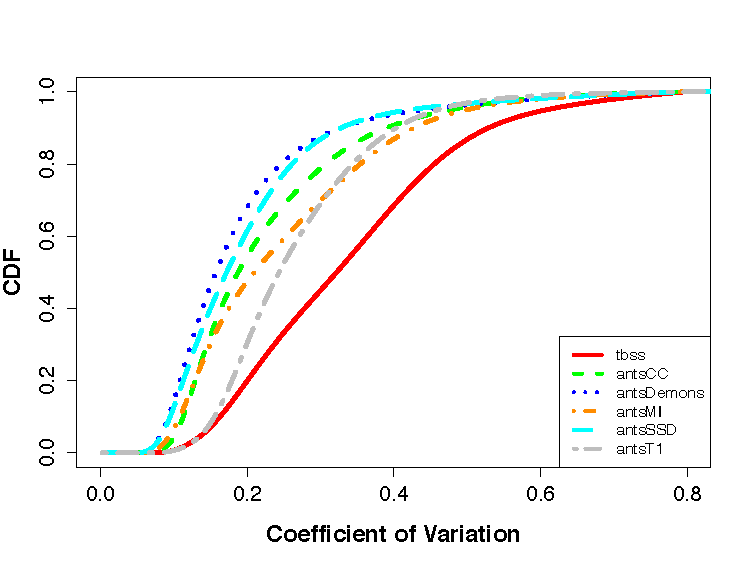
\includegraphics[width=85mm]{tbiCoV.jpg}
\end{tabular}
\caption{Comparison of the different alignment strategies in normalizing the TBI data to the FMRIB58 template.  Assessment is quantitated using the voxelwise coefficient of variation of the FA.  TBSS and the 4 ANTs metric
results were all obtained using direct registration involving subject FA and the FMRIB58 template.  The curve denoted as ``antsT1'' was also obtained in FMRIB58 space with the following transformation composition: subject FA $\rightarrow$ subject T1 $\rightarrow$ group T1 template $\rightarrow$ 
common T1 template $\rightarrow$ MNI152 (FMRIB58) template. }
\label{fig:tbi_cov}
\end{center}
\end{figure}

\begin{figure}
\begin{center}
\begin{tabular}{c}
  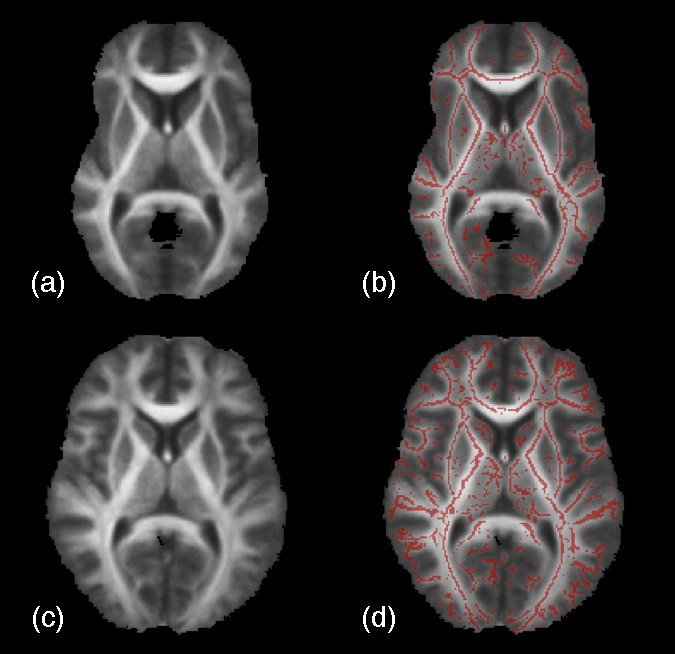
\includegraphics[width=85mm]{meanFA.jpg}
\end{tabular}
\caption{Qualitative comparison of mean FA images used in TBSS taken from the TBI data described in Section 2.  The mean FA image illustrated in (a) is created by mapping the sample FA population to the default FMRIB58 template which is the standard protocol for TBSS.  In comparison, the mean template represented in (c) is created from alignment of the population sample to the optimal T1 template as described in the paper. The respective skeleton masks in (b) and (d) are created by thresholding the resulting skeleton values $\geq 0.2$.  }
\label{fig:meanFA}
\end{center}
\end{figure}


%
%Comparison of areas of significant difference between the two groups for both methodologies can be seen on several corresponding axial slices in Fig. \ref{fig:hoonData}.  The majority of the areas of significance overlap between the two analyses although the yellow arrow points to one difference situated in the right frontal lobe.  


%As an additional quantitative comparison, we calculated the volumetric ratio between areas of significance and the volumetric brain mask for both $p = 0.01$ and $p = 0.05$.  For standard TBSS, the MNI 152 "first brain mask" was used and for the ANTs template, Atropos was used to obtain a mask by skull stripping of the final template.  These values are given in Table \ref{table:hoon}.
%
%
%\begin{table}
%  \caption{Volumetric ratio differences between ANTsTBSS and TBSS.}
%  \label{table:hoon}
%  \begin{tabular*}{88mm}{@{\extracolsep{\fill}} cccc}
%  \hline
%  {} & $\frac{V(\mathrm{mean\,FA\,mask})}{V(\mathrm{brain\,mask})}$ & $\frac{V(\mathrm{sig.\,areas})}{V(\mathrm{mean\,FA\,mask})}$ & $\frac{V(\mathrm{sig.\,areas})}{V(\mathrm{brain\,mask})}$ \\
%  \hline
%  $p \leq 0.01$ & {} & {} & {} \\
%  $p \leq 0.05$ & {} & {} & {} \\
%  \hline
%  \hline
%  \end{tabular*}
%\end{table} 





%\begin{figure}
%\begin{tabular}{c}
%  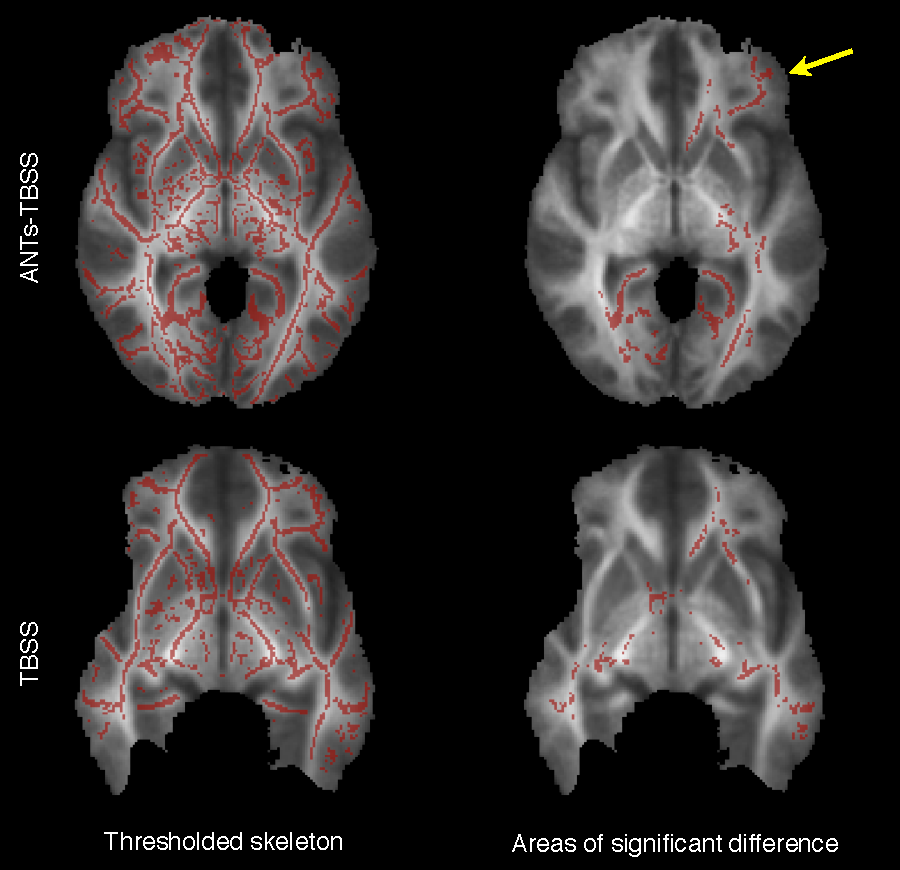
\includegraphics[width=80mm]{hoonData2.jpg}
%\end{tabular}
%\caption{Results of TBSS analysis using both the ANTs template-based approach (top row) and the standard TBSS protocol (bottom row).  Axial slices were chosen based on visual assessment of correspondence in both the ANTs template and MNI 152 template.
%On the left is the thresholded skeleton overlaid on the mean FA image.  
%On the right, significant areas of difference are given in red ($p \leq 0.01$ after the threshold-free cluster enhancement correction described in \cite{Smith2009}).  The yellow arrow points to an area of significant difference in the peripheral white matter found using ANTs-TBSS.
%}
%\label{fig:hoonData}
%\end{figure}

\subsection{INDI NKI/Rockland Sample}
In this section, further exploration of relevant issues employs 
the NKI/Rockland sample of the INDI database.  
The first is one of experimental set-up consideration in which 
we investigate how template-based
alignment is affected by the number of subject images used to 
create the template.  Both FA and mean diffusivity (MD) images were used.
This is followed by statistical analysis
of discriminating power of gender FA differences using 
the various alignment strategies.


\subsubsection{Alignment Assessment of Template Group Size}

 \begin{figure}
  \begin{center}
\begin{tabular}{c}
  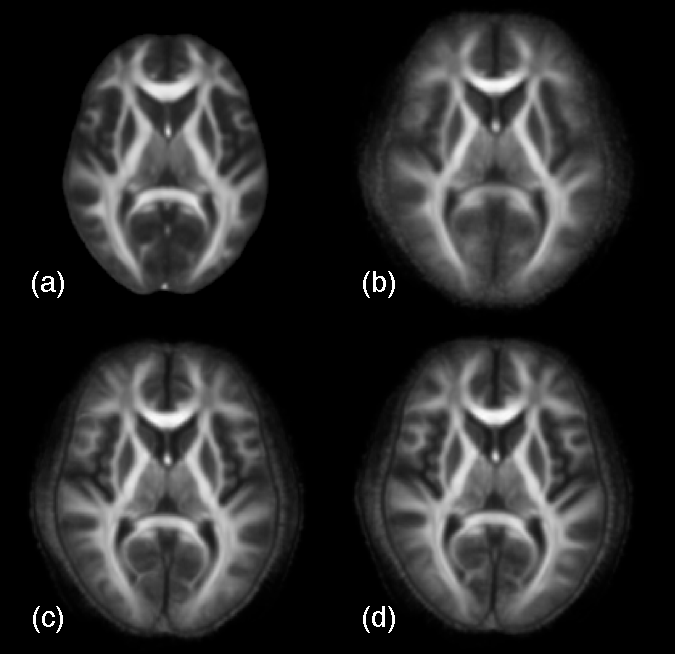
\includegraphics[width=85mm]{NKI2.jpg}
\end{tabular}
\caption{Axial slice 80 of FA mean images used in the NKI alignment assessment.  (a) The standard FMRIB58 template. (b) The mean FA image of all aligned 57 NKI data using the TBSS default FLIRT/FNIRT parameters optimized for registration to (a).  
(c) and (d) The mean FA image produced using the ANTs template-based strategy employing 5 and 30 randomly chosen subjects, respectively, warped to the space of (a) followed by T1 registration of all subjects to the resulting anatomical template.  Note the visual alignment difference particularly in the peripheral white matter complex.
}
\label{fig:NKI}
\end{center}
\end{figure}

Four templates were generated from $\{5,10,20,30\}$ randomly selected subjects 
to see if the number of subjects comprising the template affected the alignment 
performance. In addition to the composite transforms
 to take each subject's FA or MD image to the population-specific anatomical template, we also registered
each ANTs T1 template to the MNI152 template.  
This permitted a
standard space for qualitative and quantitative comparison with TBSS-aligned
FA and MD images.  
After template construction, the remaining
images were registered to the resulting template and, ultimately, 
to the MNI152 (FMRIB58) template via the template-to-MNI152 transformation.  


Sample axial slices for the FA FMRIB58-aligned mean images for the NKI data 
set of template sizes of 5 and 30 images are provided in Fig. \ref{fig:NKI}.  
We also include the same axial slice  of the FMRIB58 template in Fig. \ref{fig:NKI} 
(a) for comparison.  In both sets of sample slices, visual inspection would seemingly 
indicate better 
performance with the ANTs-based FA mean images compared with the standard 
TBSS-produced FA mean image.  Also, there is little discernible difference
 between the different ANTs results.  Alignment differences between the 
 approaches are particularly apparent in the peripheral white matter where 
 the anatomical structure in the ANTs template-based FA mean images is visually differentiable.

Relative performance is quantified in the plots produced in Fig. \ref{fig:NKIplots}. 
The mean FA image derived from the standard TBSS approach was thresholded at FA $\geq 0.2$. 
 This binary mask obtained in the NKI cohort provided the standard group mask for 
 fair comparisons for all evaluations.    For all FMRIB58-aligned images the coefficient of 
 variation (CoV) was calculated in a voxel-wise fashion within the mask.  Intuitively, 
 one would expect a smaller variance across better aligned sets of voxel values thus 
 producing a lower CoV for a given mean value.  By calculating the CDF of the set of CoV values within the mask, quantitative assessment of alignment performance can be visualized.  
% In addition to producing CDF plots for voxels within the entire brain mask, we separated the brain into inner and outer sections to investigate the alignment difference between these two regions.  This division was accomplished by applying a distance transform \cite{Maurer2003} to the FSL-provided MNI152 brain mask and thresholding the result such that the outer 30 mm form the outer mask and the subtracted binary image forms the inner mask.  Note that only those voxels that were also within the thresholded FA mask were considered in the inner/outer analysis.


There is a visible improvement in alignment for both data sets using the ANTs-based approach over individual subject FA registration to the FMRIB template.  There is little difference between the ANTs results with only a slight trend in improved performance with the larger template subject sample sizes.  
%This was the case for all three regional CoV calculations for both data sets.  Also, as expected, there is greater misalignment in the outer region versus the inner core of the white matter mask regardless of methodology.  However, the performance tally was the same in both the inner and outer regions as was the case with the entire white matter mask.% although the disparity in performance was much less for the NYU data set as the NKI data set most likely due to the differences in resolution of the original DTI.

%The improvements seen in the CDF plots are also supported by comparative quantities derived from the skeletons of the different mean FA images.  Since the skeletonization process is meant to determine the center of the various white matter tracts \cite{Smith2006}, a greater volume of skeletonization voxels would indicate identification of more centers of white matter tracts.  In addition, as described in \cite{Zalesky2011}, the number of connected components of the white matter skeleton is directly related to the contiguity and thus inversely related to the level of structure.  Table \ref{table:vol} provides the volume of the mean FA skeletons (thresholded at FA $\geq 0.2$) for standard TBSS protocol using the FMRIB template and the ANTs approach using the various templates.  In agreement with the CDF plots illustrating improved alignment with ANTs, the voxel volumes of the skeletons are greater using ANTs templates with the greatest difference seen in the outer portion of the white matter.
%Related, in Table \ref{table:cc}, we provide the number of connected components for both data sets for all isolated components greater in size than 1 voxel and 2 voxels.  Even though the skeletal volumes associated with the ANTs approach are greater, the number of connected components is less which would also support the observation of improved alignment.


%\begin{table}
%  \caption{Volume (in voxels) of thresholded mean FA skeletons.}
%  \label{table:vol}
%  \begin{tabular*}{88mm}{@{\extracolsep{\fill}} ccccc}
%  \hline
%  {} & \multicolumn{2}{c}{NKI} & \multicolumn{2}{c}{NYU} \\
%  \cline{2-5}
%  {} & inner & outer & inner & outer \\
%  \hline
%  FMRIB & 84899 & 122306 & 72765 & 76769 \\
%  ANTs$_5$ & 87572 & 134421 & 73650 & 94177 \\
%  ANTs$_{10}$ & 86908 & 130569 & 73419 & 98014 \\
%  ANTs$_{20}$ & 86523 & 129729 & 73577 & 95484 \\
%  ANTs$_{30}$ & 86971 & 128892 & 73443 & 94862 \\
%  \hline
%  \hline
%  \end{tabular*}
%\end{table} 
%
%\begin{table}
%  \caption{Number of connected components of thresholded mean FA skeletons.}
%  \label{table:cc}
%  \begin{tabular*}{88mm}{@{\extracolsep{\fill}} ccccc}
%  \hline
%  {} & \multicolumn{2}{c}{NKI} & \multicolumn{2}{c}{NYU} \\
%  \cline{2-5}
%  {} & $\geq$ 1 voxel & $\geq$ 2 voxels & $\geq$ 1 voxel & $\geq$ 2 voxels \\
%  \hline
%  FMRIB & 4340 & 1802 & 2431 & 993 \\
%  ANTs$_5$ & 3561 & 1384 & 2278 & 916 \\
%  ANTs$_{10}$ & 3413 & 1302 & 2232 & 899 \\
%  ANTs$_{20}$ & 3283 & 1252 & 2093 & 885 \\
%  ANTs$_{30}$ & 3114 & 1243 & 2128 & 867 \\
%  \hline
%  \hline
%  \end{tabular*}
%\end{table} 


%Since our proposed modification of TBSS impacts strictly the
%critical alignment step, the first set of evaluations demonstrates
%the difference between the two methods, i.e. spatial normalization 
%via registration of the FA maps to the FMRIB58 template
%or spatial normalization via ANTs template construction.  

%It is important to note that we did not consider normalization either to a random subject
%or to the subject best representative of the mean as defined in 
%\cite{Smith2006}. The former was not investigated due to the possible bias
%in selecting a random subject as described in \cite{Smith2006}.  
%Neither was the latter option pursued due to the computational complexity
%required for such an $\OO{n^2}$ search over the relatively large NKI data set.  In addition, normalization to
%the FMRIB58 template is both the default and recommended option
%with the parameters of FNIRT optimally tuned for said option.  

%To warp the MD images following FA registration we used FSL's {\bf applywarp} function using the FA-derived transform. 

%\begin{figure}
%\begin{tabular}{c}
%  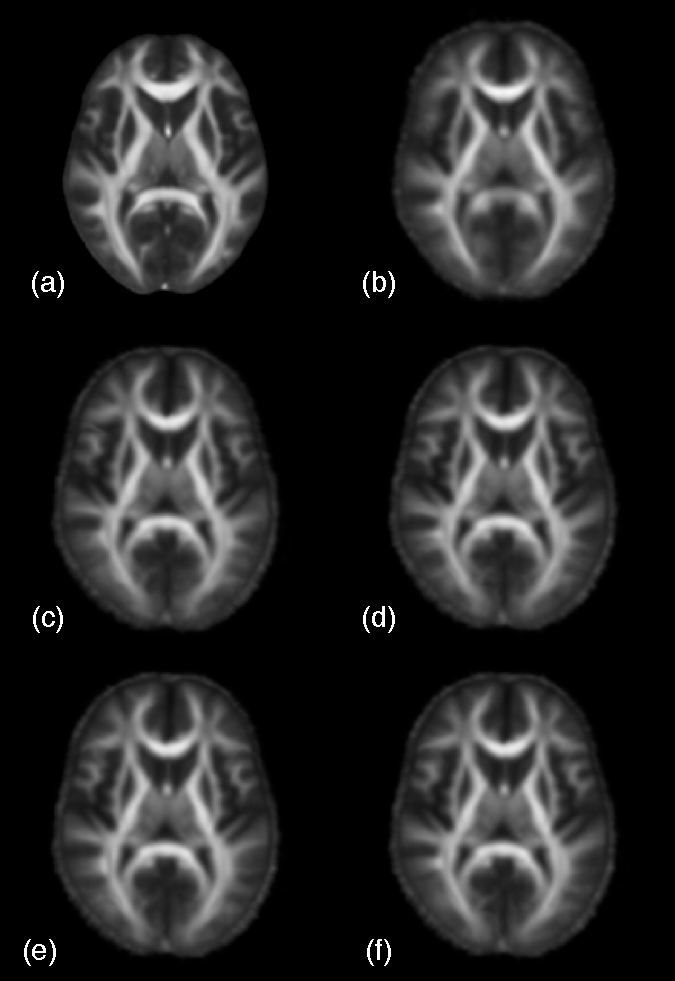
\includegraphics[width=80mm]{NYU.jpg}
%\end{tabular}
%\caption{Axial slice 80 of FA mean images used in the NYU alignment assessment.  (a) The standard FMRIB58\_FA\_1mm template. (b) The mean FA image of all aligned 57 NKI data using the TBSS default FLIRT/FNIRT parameters optimized for registration to (a).  
%(c)-(f) The mean FA image produced using the ANTs template-based strategy employing 5, 10, 20, and 30 randomly chosen subjects, respectively, warped to the space of (a).  Note the visual alignment difference particularly in the peripheral white matter complex.
%}
%\label{fig:NYU}
%\end{figure}








 
%\begin{figure}
%\begin{tabular}{c}
%  \includegraphics[width=80mm]{inner.png}
%\end{tabular}
%\caption{
%}
%\label{fig:inner}
%\end{figure}
%
%\begin{figure}
%\begin{tabular}{c}
%  \includegraphics[width=80mm]{outer.png}
%\end{tabular}
%\caption{Three-canonical view of the inner
%}
%\label{fig:outer}
%\end{figure}

%\begin{figure*}
%\begin{tabular}{c}
%  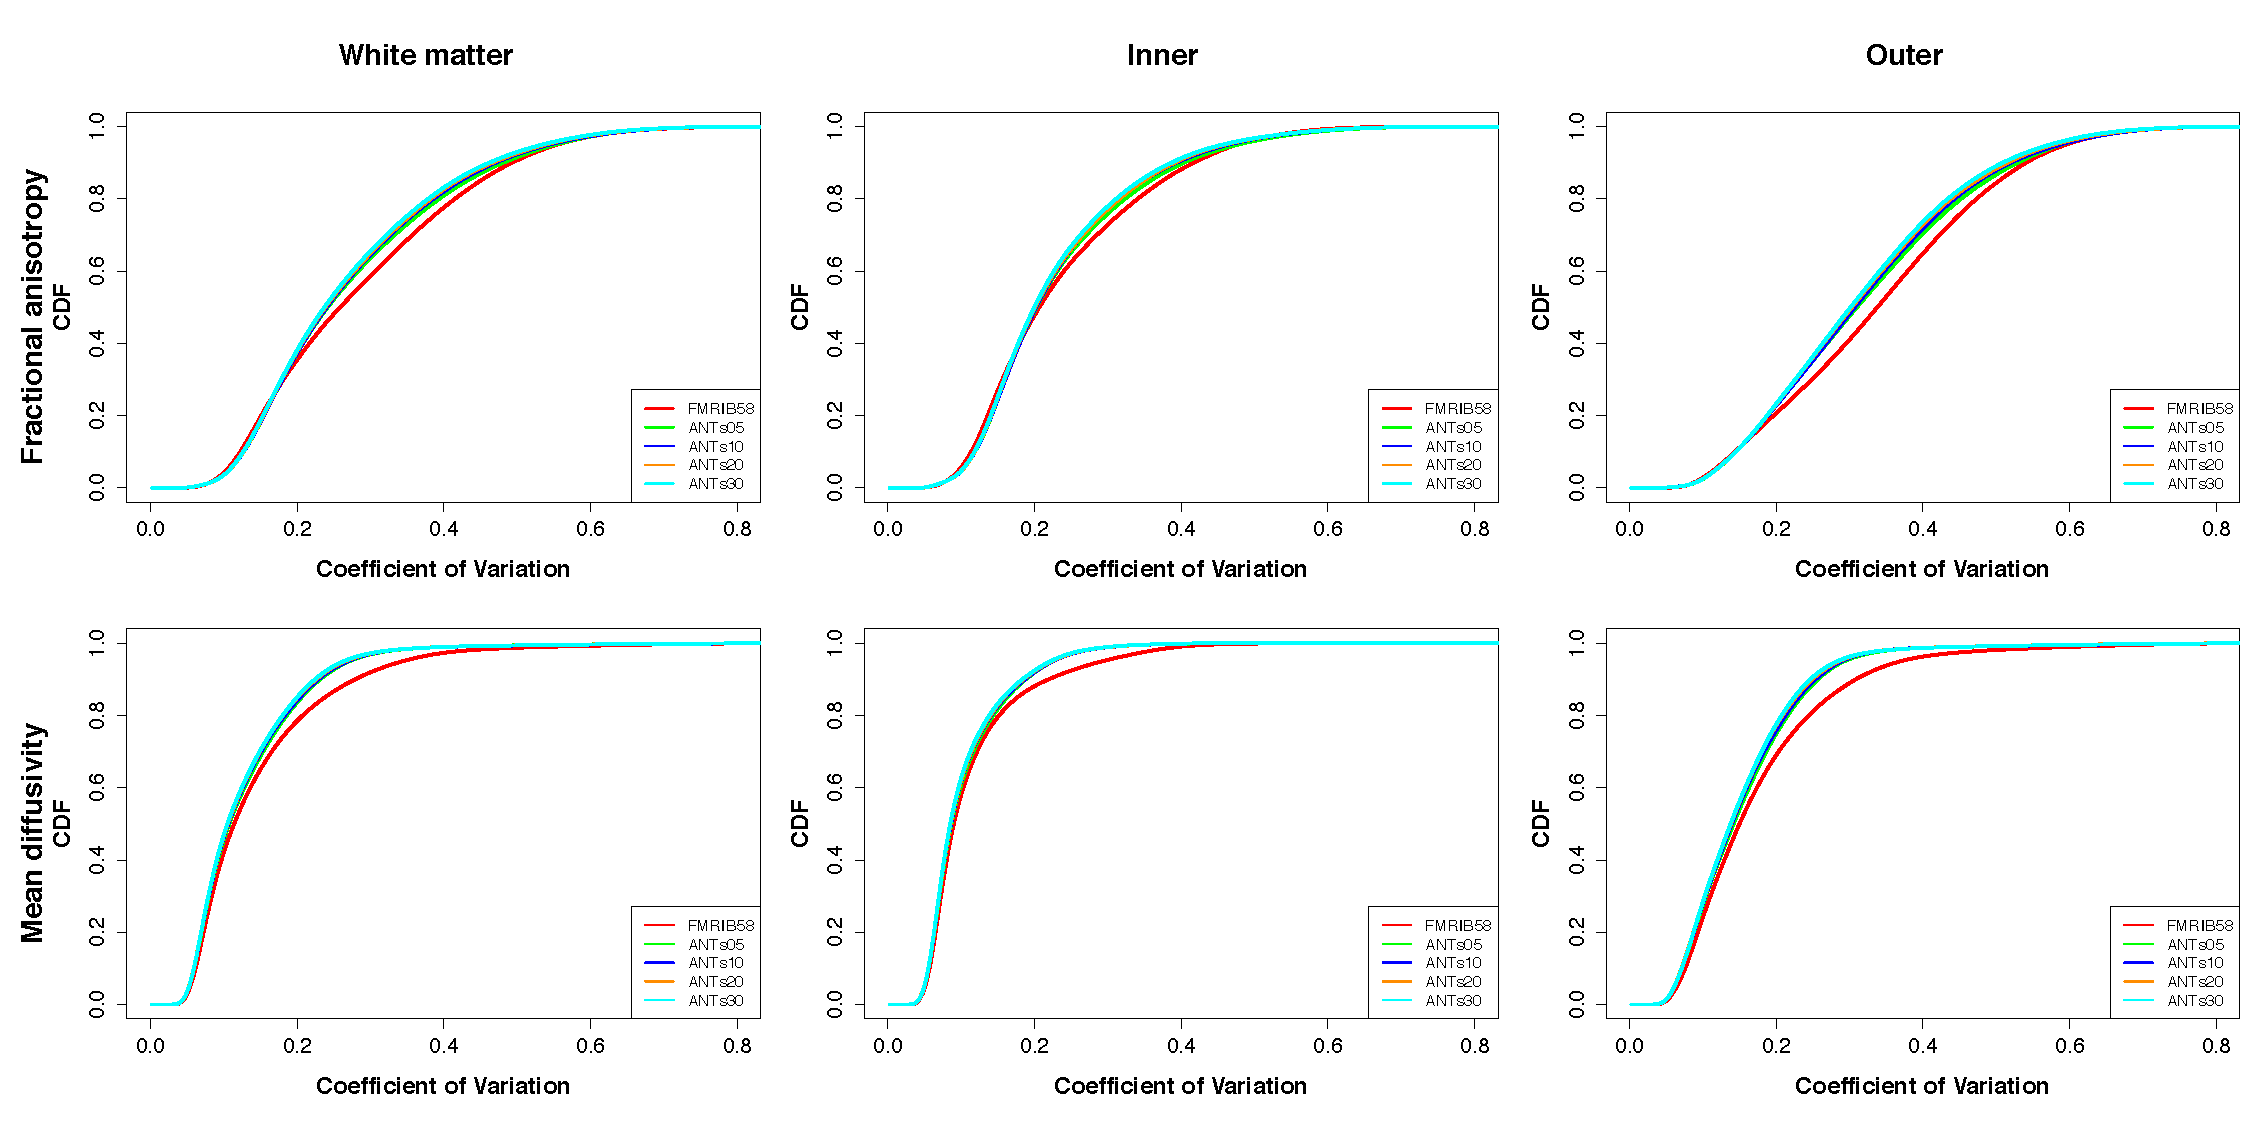
\includegraphics[width=180mm]{NYUplots2.jpg}
%\end{tabular}
%\caption{{\bf NYU alignment assessment:}  To compare alignments between the  standard TBSS approach of using the FMRIB58 template versus using the different ANTs templates, we calculated the coefficient of variation at each voxel (for both FA and MD) and plotted the CDF over the range of values $[0,0.8]$ accumulated over all the voxels inside the thresholded (FA $\geq 0.2$) standard TBSS mean FA image (see Fig. \ref{fig:NKI}(b)).  In addition to the whole brain analysis (first column), the coefficient of variation was separately calculated over the inner and outer portions of the white matter (second and third columns, respectively).  The CDF plots for the ANTs templates are all very similar (although trending towards slight improvement with larger template sample size) and illustrate the general improvement in FA and MD alignment over registration of each FA image to the FMRIB58 template.
%}
%\label{fig:NYUplots}
%\end{figure*}


\begin{figure}
\begin{tabular}{c}
  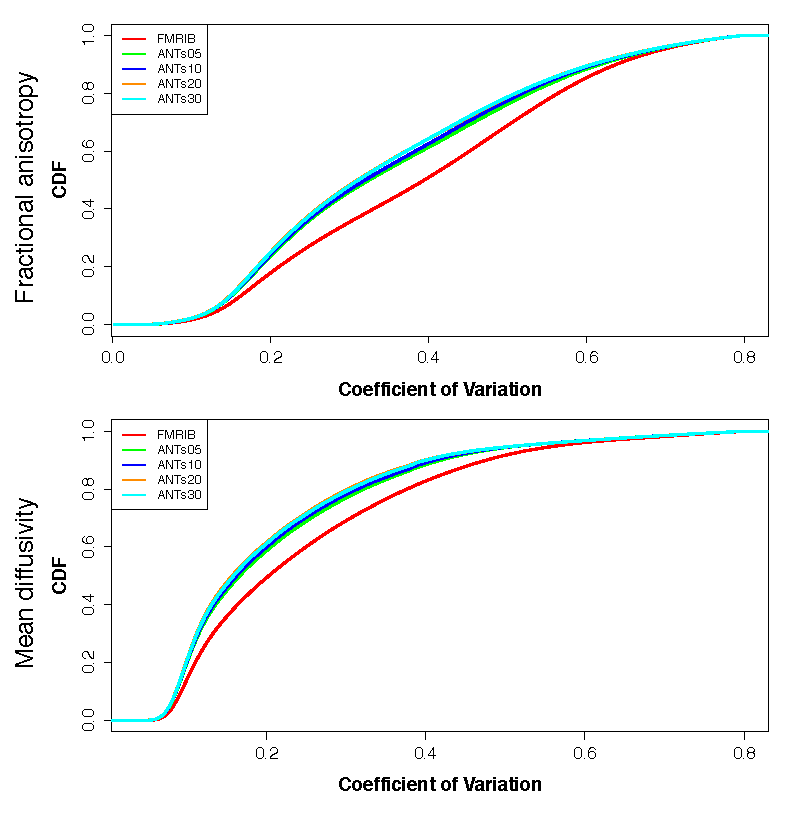
\includegraphics[width=85mm]{NKIplots3.jpg}
\end{tabular}
\caption{{\bf NKI alignment assessment:}  To compare alignments between the  standard TBSS approach of using the FMRIB58 template versus using the different ANTs templates, we calculated the coefficient of variation at each voxel (for both FA and MD) and plotted the CDF over the range of values $[0,0.8]$ accumulated over all the voxels inside the thresholded (FA $\geq 0.2$) standard TBSS mean FA image (see Fig. \ref{fig:NKI}(b)).  The CDF plots for the ANTs templates are all very similar (although trending towards slight improvement with larger template sample size) and illustrate the general improvement in FA and MD alignment over registration of each FA image to the FMRIB58 template.
}
\label{fig:NKIplots}
\end{figure}


\subsubsection{Statistical Power Related to Gender-Based FA Differences}

For completeness, the second NKI data subset was used to explore the 
power of the different alignment strategies in discriminating FA 
differences in a control group divided by gender.  As described 
earlier, this group consisted of 27 subjects 
comprised of 9 females (age: $29.3 \pm 6.6$ years) and 18 males (age: $26.6 
\pm 6.9$ years).  Each subject was registered to the template made from 
30 randomly chosen subjects, described in the previous section, and
subsequently warped to the MNI152 template space.  

Results are shown in Fig. \ref{fig:nki_testing} in which all but the more
robust metrics (MI and CC) exhibit similar power.  Note that the magnitude
of the effects is much smaller than for TBI.  Again, the template-based approach
performs comparatively well without the negative effects associated with
the issues perviously described.

\begin{figure*}
\begin{center}
\begin{tabular}{c}
  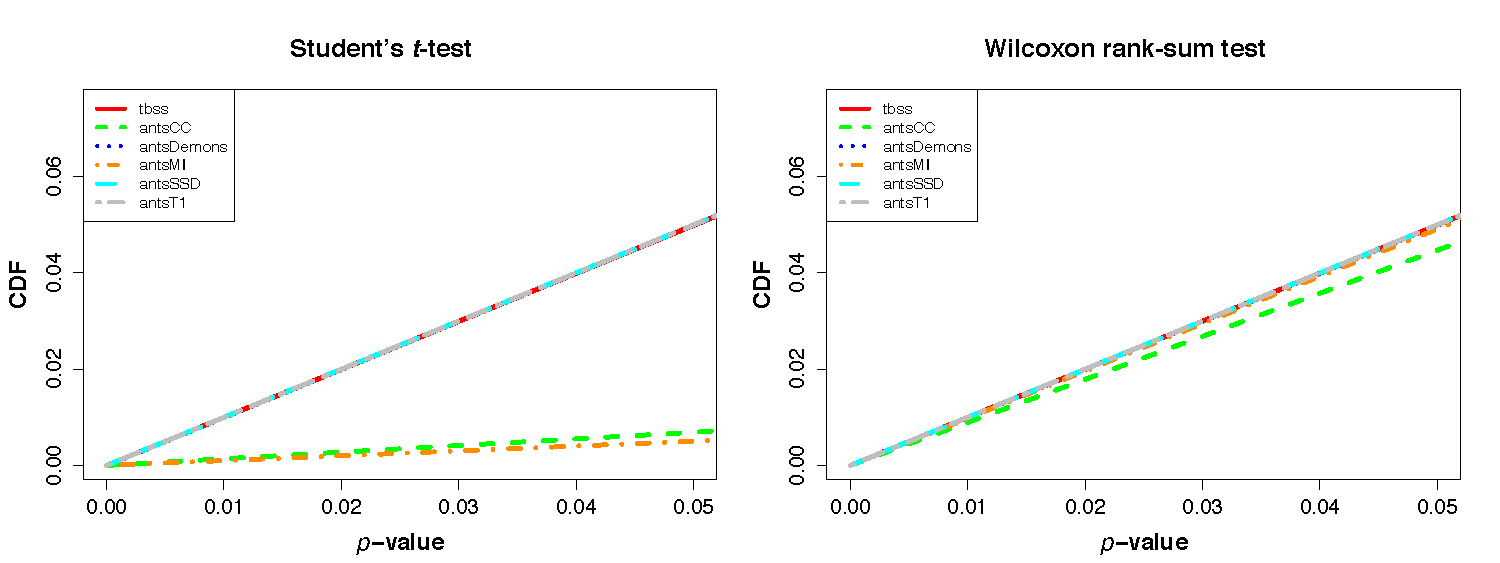
\includegraphics[width=180mm]{nkiTesting.jpg}
\end{tabular}
\caption{Student's $t$-test and the nonparametric Wilcoxon rank-sum test results 
(one-tailed, $\alpha = 0.95$) for the NKI FA data aligned to the FMRIB58 template 
adjusted for multiple comparisons (FDR).  
Similar statistical power is seen in all alignment scenarios except for the more robust
metrics (CC and MI) in the $t$-test which show decreased power.   }
\label{fig:nki_testing}
\end{center}        
\end{figure*}


%\section{Discussion}
%This should explore the significance of the results of the work, not repeat them. A combined Results and Discussion section is often appropriate. Avoid extensive citations and discussion of published literature.

\section{Discussion} Prior evaluation work using anatomically labeled
data indicates that mutual information,
cross-correlation and the SSD/Demons metric are all capable of producing
high quality anatomical alignment (e.g. \cite{Klein2009}).  All of this work, though, compares
the quality of alignment at a relatively coarse scale of major gyri,
lobes and regions.  At the voxel level, it is nearly impossible to
determine the ground truth correspondence.  Indeed, there is no reason
to believe that subtle differences between a set of alignment strategies
(induced, in the experiments of this paper, by changing the similarity
metrics used in image registration) that all apparently work well should
be considered significant.  This work, however, highlights a dramatic impact of similarity metric choice on detection power in template-based FA studies.  Our contention is that this dramatic "improvement" in detection power is not due to better anatomical alignment.  Rather, it is a result of circularity/nonindependence of the normalization and statistical estimation strategy.  Consequently, we recommend that future work should take greater care when pairing the normalization strategy with the statistical framework.  Furthermore, we recommend that researchers should diligently seek to maintain independence between these two critical stages of a population study.  That is, {the features that drive the minimization of a similarity metric should be independent of the features that will be used in hypothesis testing.  In particular, one should avoid combining the SSD metric for normalizing FA with Student's t-test for FA differences.

\section{Conclusions}
%The main conclusions of the study may be presented in a short Conclusions section, which may stand alone or form a subsection of a Discussion or Results and Discussion section.

%The popularity of FSL's TBSS is due, in large part, to its ease of use.  Anybody interested in performing a neuroimaging study in which DTI-derived measures are compared across populations can simply download FSL and immediately apply it to their data.  The proposed work is a substantial improvement to the core TBSS framework which dovetails with FSL.  In addition, it is comparably easy to download and apply what we have proposed in the form of ANTs-TBSS.  

With the increasing use of DTI for white matter assessment and the
increasing number of researchers that are taking advantage of the numerous
software tools that are available to facilitate this research, guidance
is necessary to ensure the proper use of these tools and the
calculation and reporting of findings \cite{Ridgway2008}.  The normalization 
circularity issue described in this work is the inducement of substantial Type 1
errors caused by FA-to-FA normalization using standard similarity metrics.
To reduce these types of errors, we advocate the use of an anatomical template-building
strategy whereby the transformation of FA images to a common space is performed
using each individual's anatomical image.
This proposed improvement potentially has many benefits:
%which were listed in the 
%introduction.  Such benefits range from the theoretical in the form of eliminating 
%the confounding effects of registering data which is to be statistically 
%differentiated to the practical, e.g. reusing the ANTs-based template for other 
%neuroimaging analyses.  
\begin{itemize}
\item As explained in \cite{Avants2010}, ANTs optimal template construction creates a true Frech\'et mean from the population sample with high resolution which facilitates within-group registration.  This obviates the need for an externally-derived template or an $\OO{n^2}$ search for an approximation to the mean subject or the bias resulting from random subject selection.
\item Since the creation of the standardized coordinate system is performed using the anatomical images, nonrigid registration of the DTI-derived scalar images is 
minimized thus mitigating the confounds described previously.  Each DTI-based image is rigidly registered to its corresponding T1 image followed by a small number of nonrigid registration iterations to account for echo planar imaging (EPI) distortion \cite{Wu2008}.  
\item Although the total number of registrations to be performed is increased, this makes the composite registration between an individual DTI-derived image to the template more robust as the shape distance between registrations is minimized.
%\item Instead of Gaussian smoothing as with SPM, TBSS uses the warping process to FMRIB58 by default to provide an indirect smoothing.  Such resampling occurs in ANTs-TBSS as a by-product of the registration of the DTI-derived image to the corresponding T1 image in a subject-specific manner.
%\item Instead of using thresholding to create the white matter segmentation from which the skeleton is created, an anatomically-based segmentation, either in the template space or in each subject space followed by a label fusion technique (e.g. majority voting), can be used to ultimately provide a more accurate skeleton.
\item Oftentimes FA analysis is only one of several components performed in a population-based study.  Other investigations, such as voxel- and tensor-based morphometry, cortical thickness measurements, etc. can take advantage of the anatomical template.
\item The proposed modification is compatible with other frameworks such as TBSS where the normalization step is
performed using ANTs-based tools followed by skeletonization and projection using the FMRIB software (see Fig. \ref{fig:workflow}).
\end{itemize}

Of practical significance, we emphasize that all software components described 
in this paper are publicly available as open source primarily through the 
Advanced Normalization Tools (ANTs) repository.%
\footnote{
http://www.picsl.upenn.edu/ANTs
}
In addition to registration and template building, ANTs also includes brain 
extraction \cite{Avants2010a}, bias correction \cite{Tustison2010}, $n$-tissue 
segmentation \cite{Avants2011a}, and cortical thickness estimation solutions \cite{Das2009}.  


%In performing the various analyses described in the work, it was pleasantly surprising to discover how well the alignments were for the ANTs template data considering that alignment was based on FA-to-FA correspondence and no such image registrations were performed to align FA directly with FA as with TBSS.  Furthermore, since TBSS is a local quantification method with increased statistical power through the use of the skeletonization and projection step, improved alignments can increase the regional sensitivity to local white matter differences particularly in the peripheral tracts.

%% The Appendices part is started with the command \appendix;
%% appendix sections are then done as normal sections
%% \appendix

%% \section{}
%% \label{}

%% References
%%
%% Following citation commands can be used in the body text:
%% Usage of \cite is as follows:
%%   \cite{key}          ==>>  [#]
%%   \cite[chap. 2]{key} ==>>  [#, chap. 2]
%%   \citet{key}         ==>>  Author [#]

%% References with bibTeX database:

\section*{Acknowledgments}
All visualizations were performed using ITK-SNAP%
\footnote{
http://www.itksnap.org/
}
\cite{Yushkevich2006} and
DTI-TK.%
\footnote{
http://www.nitrc.org/projects/dtitk/
}
We also gratefully acknowledge Dr. Niels van Strien of the Norwegian University of Science and Technology
who packaged the template construction algorithm in the very useful script \verb#buildtemplateparallel.sh#
which is publicly available in ANTs.

\section*{References}

\bibliographystyle{elsarticle-harv}
\bibliography{references}


%% Authors are advised to submit their bibtex database files. They are
%% requested to list a bibtex style file in the manuscript if they do
%% not want to use model1-num-names.bst.

%% References without bibTeX database:

% \begin{thebibliography}{00}

%% \bibitem must have the following form:
%%   \bibitem{key}...
%%

% \bibitem{}

% \end{thebibliography}


\end{document}

%%
%% End of file `elsarticle-template-1-num.tex'.
